\documentclass[journal]{IEEEtran}
\PassOptionsToPackage{x11names}{xcolor}

% packages
\usepackage{hyperref}
\usepackage{flushend}
\usepackage[inline]{enumitem}
\usepackage{array,multirow,graphicx}
\usepackage{float}
\usepackage{cite}
\usepackage{bm}
\usepackage{orcidlink}

\usepackage{xcolor}
% \usepackage{microtype,xparse,tcolorbox}

%% footnote
\usepackage{footnote}
\makesavenoteenv{tabular}
\makesavenoteenv{table}
\makesavenoteenv{tabular*}
\makesavenoteenv{table*}
% \usepackage{tablefootnote}

%% graphics packages
\usepackage{tikz}
\usepackage{pgfplots}
\usetikzlibrary{patterns}
    \pgfplotsset{compat=1.15}
\usepackage{colortbl}
\usepackage{graphicx}
\usepackage{multirow}
\usepackage{circuitikz}
\usepackage{dblfloatfix}
\usepackage[bottom]{footmisc}
\ifCLASSOPTIONcompsoc
    \usepackage[caption=false, font=normalsize, labelfont=sf, textfont=sf]{subfig}
\else
    \usepackage[caption=false, font=footnotesize]{subfig}
\fi

%% checkmark packages 
\usepackage{pifont}
\newcommand{\cmark}{\ding{51}}
\newcommand{\xmark}{\ding{55}}

%% math packages
\usepackage{amssymb}
\usepackage{amsmath}
\usepackage{mathtools}
\usepackage{booktabs}

% math 
\IEEEeqnarraydefcolsep{0}{\hoffset}
\newcommand*{\defeq}{\stackrel{\text{def}}{=}}

% definition setup
%\theoremstyle{definition}

\newtheorem{defn}{Definition}[section]

% text that may be removed to reach the 10-page limit
\newcommand{\removable}[1]{{\color{red}#1}}
% placeholder for input after the Harmonic Meeting of 30/10
\newcommand{\placeholder}[1]{\textcolor{blue}{[#1]}}

% correct bad hyphenation here
\hyphenation{op-tical net-works semi-conduc-tor}

% document
\begin{document}

% title, authors and thanks
\title{Stochastic Harmonic Hosting Capacity \\ Considering Harmonic Recombination}
\author{Tom~Van~Acker~\orcidlink{0000-0001-6283-1457},%
        Jinwen~Xiang~\orcidlink{0000-0003-2107-0238},%
        and~Hakan~Ergun,~\IEEEmembership{Senior Member,~IEEE~\orcidlink{0000-0001-5171-1986}}%
\thanks{Tom Van Acker is with the Scenarios, Markets and Adequacy Department, Elia Transmission Belgium, 1000 Brussels, Belgium (e-mail: tom.vanacker@elia.com).}%
\thanks{Jinwen Xiang and Hakan Ergun are with the Research Group ELECTA, Department of Electrical Engineering, KU Leuven, 3000 Leuven, Belgium, and also with Etch-EnergyVille, 3600 Genk, Belgium (e-mail: jinwen.xiang@kuleuven.be, hakan.ergun@kuleuven.be).}
\thanks{This work is supported by the Energy Transition Fund by FOD Economy, Belgium, project HARMONIC. The General Board on Energy of the FOD Economy is not liable for any use of the presented work and subsequent results.}
\thanks{\textit{(Corresponding author: Tom~Van~Acker)}}}

% paper headers
\markboth{Journal of \LaTeX\ Class Files,~Vol.~14, No.~8, August~2015}%
{Shell \MakeLowercase{\textit{et al.}}: Bare Demo of IEEEtran.cls for IEEE Journals}

% make the title area
\maketitle

% abstract
\begin{abstract}
The aggregation of harmonic currents from many power-electronic interfaced units depends on their phase angles, which are uncertain at the planning stage. This paper presents a stochastic harmonic hosting capacity method for phase-balanced three-phase power systems that captures harmonic recombination. The angle uncertainty is characterized through a harmonic state-space model and is represented by polynomial chaos expansion, with one random variable per unit and one shared by all units of a converter type, and the angles are referenced to each unit's fundamental terminal voltage. Harmonic voltage and current limits are enforced through chance constraints. For fairness criteria that fix the ratios between the allocations of the units, e.g., absolute equality, the problem reduces to a small second-order cone program that equals the general formulation and recovers the deterministic hosting capacity exactly when the uncertainty vanishes. For the IEEE 30-bus system, recombination between units of a single converter type is limited, and the indicative summation exponents of IEC~61000-3-6 overestimate the hosting capacity by a factor of about two, irrespective of added capacitor banks or underground cables. A mix of four or more converter types raises the hosting capacity by about 80\,\% and brings the low-order summation exponent to the indicative value, and the choice of the stochastic bound changes the hosting capacity by up to 38\,\%.
\end{abstract}

% keywords
\begin{IEEEkeywords}
Chance constraints, harmonic distortion, harmonic recombination, hosting capacity, polynomial chaos expansion.
\end{IEEEkeywords}

% peer-review title
\IEEEpeerreviewmaketitle

% sections
% % Math Operators
% \DeclareMathOperator{\rank}{rank}
% \DeclareMathOperator{\diag}{diag}
% \DeclareMathOperator{\diagm}{diagm}
% \DeclareMathOperator{\real}{Re}
% \DeclareMathOperator{\imag}{Im}
% \DeclareMathOperator{\trace}{tr}
% \DeclareMathOperator{\sign}{sign}
% \DeclareMathOperator{\subjectto}{s.t.}
% \DeclareMathOperator{\matr}{mat}
% \DeclareMathOperator{\vecr}{vec}
% \DeclareMathOperator{\atantwo}{atan2}
% \DeclareMathOperator{\postproc}{post}
% \DeclareMathOperator{\preproc}{pre}
% \DeclareMathOperator{\vars}{var}

% Time
\newcommand{\Time}{t}
\newcommand{\Period}{T}

% Numbers
\newcommand{\NaturalNumberSet}{\mathbb{N}}
\newcommand{\RealNumberSet}{\mathbb{R}}
\newcommand{\ComplexNumberSet}{\mathbb{C}}

% Vector
\newcommand{\im}{j}

% Random Variables and Moments
\newcommand{\RVX}{\mathsf{x}}
\newcommand{\RVY}{\mathsf{y}}
\newcommand{\RVZ}{\mathsf{z}}
\newcommand{\ApproxRVX}{\hat{\RVX}}
\newcommand{\ApproxRVY}{\hat{\RVY}}
\newcommand{\ApproxRVZ}{\hat{\RVZ}}
\newcommand{\Probability}{\mathbb{P}}
\newcommand{\Expectation}{\mathbb{E}}
\newcommand{\Variance}{\mathbb{V}}
\newcommand{\Skewness}{\mathbb{S}}
\newcommand{\Kurtosis}{\mathbb{K}}

% Sets and Indices
\newcommand{\Node}{i}
\newcommand{\AltNode}{j}
\newcommand{\NodeSet}{\mathcal{I}}
\newcommand{\RefNodeSet}{\NodeSet^{\text{ref}}}
\newcommand{\Edge}{e}
\newcommand{\EdgeSet}{\mathcal{E}}
\newcommand{\Line}{b}
\newcommand{\LineSet}{\mathcal{B}}
\newcommand{\Unit}{u}
\newcommand{\UnitSet}{\mathcal{U}}
\newcommand{\PCEIndex}{k}
\newcommand{\PCESet}{\mathcal{K}}
\newcommand{\FixedUnitSet}{\UnitSet^{\text{f}}}
\newcommand{\HarmonicUnitSet}{\UnitSet^{\text{h}}}
\newcommand{\DispatchableUnitSet}{\UnitSet^{\text{d}}}
\newcommand{\Harmonic}{h}
\newcommand{\HarmonicSet}{\mathcal{H}}
\newcommand{\PositiveHarmonicSet}{\HarmonicSet^{\texttt{+}}}
\newcommand{\NegativeHarmonicSet}{\HarmonicSet^{\texttt{-}}}
\newcommand{\ZeroHarmonicSet}{\HarmonicSet^{\texttt{0}}}
\newcommand{\Winding}{w}
\newcommand{\WindingSet}{\mathcal{W}}
\newcommand{\Xfmr}{x}
\newcommand{\XfmrSet}{\mathcal{X}}


% Union Sets and Indices
\newcommand{\TupleSet}{\mathcal{T}}
\newcommand{\LineTuple}{\Line\Node\AltNode}
\newcommand{\AltLineTuple}{\Line\AltNode\Node}
\newcommand{\EdgeTuple}{\Edge\Node\AltNode}
\newcommand{\AltEdgeTuple}{\Edge\AltNode\Node}
\newcommand{\EdgeTupleSet}{\TupleSet^{\text{\Edge}}}
\newcommand{\EdgeTupleSetFr}{\TupleSet^{\text{\Edge}\Arrow{.15cm}}}
\newcommand{\EdgeTupleSetTo}{\TupleSet^{\text{\Edge}\Arrowright{.15cm}}}
\newcommand{\LineTupleSet}{\TupleSet^{\text{\Line}}}
\newcommand{\LineTupleSetFr}{\TupleSet^{\text{\Line}\Arrow{.15cm}}}
\newcommand{\LineTupleSetTo}{\TupleSet^{\text{\Line}\Arrowright{.15cm}}}
\newcommand{\XfmrTupleSet}{\TupleSet^{\text{\Xfmr}}}
\newcommand{\XfmrTupleSetFr}{\TupleSet^{\text{\Xfmr}\Arrow{.15cm}}}
\newcommand{\XfmrTupleSetTo}{\TupleSet^{\text{\Xfmr}\Arrowright{.15cm}}}
\newcommand{\UnitTuple}{\Unit\Node}
\newcommand{\UnitTupleSet}{\TupleSet^{\text{\Unit}}}
\newcommand{\FixedUnitTupleSet}{\TupleSet^{\text{\Unit,f}}}
\newcommand{\HarmonicUnitTupleSet}{\TupleSet^{\text{\Unit,h}}}
\newcommand{\DispatchableUnitTupleSet}{\TupleSet^{\text{\Unit,d}}}

\newcommand{\Arrow}[1]{%
\parbox{#1}{\tikz{\draw[->](0,0)--(#1,0);}}
}
\newcommand{\Arrowright}[1]{%
\parbox{#1}{\tikz{\draw[<-](0,0)--(#1,0);}}
}

% Electrical Variables
%% Current
\newcommand{\Current}{\mathsf{I}}
\newcommand{\ComplexCurrent}{\mathsf{\bar{I}}}
\newcommand{\CurrentMagnitude}{\Current^{\text{mag}}}
\newcommand{\RealCurrent}{\Current^{\text{re}}}
\newcommand{\ImaginaryCurrent}{\Current^{\text{im}}}
\newcommand{\SeriesCurrent}{\Current^{\text{s}}}
\newcommand{\ComplexSeriesCurrent}{\ComplexCurrent^{\text{s}}}
\newcommand{\RealSeriesCurrent}{\Current^{\text{s,re}}}
\newcommand{\RealSeriesCurrentFrom}{\Current^{\text{s,re,fr}}}
\newcommand{\RealSeriesCurrentTo}{\Current^{\text{s,re,to}}}
\newcommand{\ImaginarySeriesCurrent}{\Current^{\text{s,im}}}
\newcommand{\ImaginarySeriesCurrentFrom}{\Current^{\text{s,im,fr}}}
\newcommand{\ImaginarySeriesCurrentTo}{\Current^{\text{s,im,to}}}
\newcommand{\ShuntCurrent}{\Current^{\text{sh}}}
\newcommand{\ComplexShuntCurrent}{\ComplexCurrent^{\text{sh}}}
\newcommand{\RealShuntCurrent}{\Current^{\text{sh,re}}}
\newcommand{\ImaginaryShuntCurrent}{\Current^{\text{sh,im}}}
\newcommand{\RealMagnetizingCurrent}{\Current^{\text{m,re}}}
\newcommand{\ImaginaryMagnetizingCurrent}{\Current^{\text{m,im}}}
\newcommand{\RealExcitationCurrent}{\Current^{\text{e,re}}}
\newcommand{\ImaginaryExcitationCurrent}{\Current^{\text{e,im}}}

\newcommand{\CurrentWave}[1]{i_{#1}(\Time)}
%% Voltage
\newcommand{\Voltage}{\mathsf{U}}
\newcommand{\ComplexVoltage}{\mathsf{\bar{U}}}
\newcommand{\RealVoltage}{\Voltage^{\text{re}}}
\newcommand{\ImaginaryVoltage}{\Voltage^{\text{im}}}
\newcommand{\ReferenceVoltage}{\Voltage^{\text{ref}}}

\newcommand{\AltVoltageVariable}{\mathsf{V}}
\newcommand{\ComplexAltVoltage}{\mathsf{\bar{V}}}
\newcommand{\RealAltVoltage}{\AltVoltageVariable^{\text{re}}}
\newcommand{\ImaginaryAltVoltage}{\AltVoltageVariable^{\text{im}}}

\newcommand{\LiftedCurrentVariable}{\mathsf{J}}
\newcommand{\LiftedCurrent}{\LiftedCurrentVariable}
\newcommand{\LiftedVoltageVariable}{\mathsf{W}}
\newcommand{\LiftedVoltage}{\LiftedVoltageVariable}

\newcommand{\VoltageWave}[1]{u_{#1}(\Time)}

%% Excitation Voltage
\newcommand{\ExcitationVoltageVariable}{\mathsf{E}}
\newcommand{\ComplexExcitationVoltage}{\mathsf{\bar{E}}}
\newcommand{\RealExcitationVoltage}{\ExcitationVoltageVariable^{\text{re}}}
\newcommand{\ImaginaryExcitationVoltage}{\ExcitationVoltageVariable^{\text{im}}}
\newcommand{\RealExcitationVoltageVector}{\overline{\ExcitationVoltageVariable}^{\text{re}}}
\newcommand{\ImaginaryExcitationVoltageVector}{\overline{\ExcitationVoltageVariable}^{\text{im}}}

%% Power 
\newcommand{\Power}{\mathsf{S}}
\newcommand{\RealPower}{\mathsf{P}}
\newcommand{\ImaginaryPower}{\mathsf{Q}}

% Electrical Parameters
%% Frequency
\newcommand{\Frequency}{f}
\newcommand{\FundamentalFrequency}{\Frequency^{\text{fund}}}
\newcommand{\AngularFrequency}{\omega}
\newcommand{\FundamentalAngularFrequency}{\AngularFrequency^{\text{fund}}}
%% Current
\newcommand{\CurrentParameter}{I}
\newcommand{\CurrentPhasor}[1]{\CurrentParameter_{#1}}
\newcommand{\SeriesCurrentPhasor}[1]{\CurrentPhasor{#1}^{\text{s}}}
\newcommand{\ShuntCurrentPhasor}[1]{\CurrentPhasor{#1}^{\text{sh}}}
\newcommand{\ExcitationCurrentPhasor}[1]{\CurrentParameter_{#1}^{\text{e}}}
\newcommand{\MagnetizingCurrentPhasor}[1]{\CurrentParameter_{#1}^{\text{m}}}
% duplicate of line 101 (an error, so pdfLaTeX already kept the first definition): \newcommand{\CurrentMagnitude}[1]{\CurrentParameter_{#1}^{\text{mag}}}
\newcommand{\RatedCurrent}{\CurrentParameter^{\text{rated}}}
\newcommand{\FundamentalCurrentMagnitude}[1]{\CurrentParameter_{#1}^{\text{mag,fund}}}

\newcommand{\CurrentAngleParameter}{\varphi}
\newcommand{\CurrentAngle}[1]{\CurrentAngleParameter_{#1}}

%% Voltage
\newcommand{\VoltageParameter}{U}
\newcommand{\MinimumVoltage}{\VoltageParameter^{\text{min}}}
\newcommand{\MaximumVoltage}{\VoltageParameter^{\text{max}}}
\newcommand{\ExtremeVoltage}{\hat{\VoltageParameter}^{\text{max}}}
\newcommand{\VoltageMagnitude}[1]{\VoltageParameter_{#1}^{\text{mag}}}
\newcommand{\FundamentalVoltageMagnitude}[1]{\VoltageParameter_{#1}^{\text{mag,fund}}}
\newcommand{\RealRefVoltage}{\VoltageParameter^{\text{ref,re}}}
\newcommand{\ImaginaryRefVoltage}{\VoltageParameter^{\text{ref,im}}}

\newcommand{\AltVoltageParameter}{V}

\newcommand{\ExcitationVoltageParameter}{E}
\newcommand{\ExcitationVoltageVector}{\overline{\ExcitationVoltageParameter}}
\newcommand{\ExcitationVoltagePhasor}[1]{\ExcitationVoltageParameter_{#1}}

\newcommand{\VoltageAngleParameter}{\theta}
\newcommand{\VoltageAngle}[1]{\VoltageAngleParameter_{#1}}

\newcommand{\VoltagePhasor}[1]{\VoltageParameter_{#1}}
\newcommand{\AltVoltagePhasor}[1]{\AltVoltageParameter_{#1}}
%% Power
\newcommand{\ApparentPowerParameter}{S}
\newcommand{\ApparentPowerPhasor}[1]{\ApparentPowerParameter_{#1}}

\newcommand{\RealPowerParameter}{P}
\newcommand{\MinimumRealPower}{P^{\text{min}}}
\newcommand{\MaximumRealPower}{P^{\text{max}}}
\newcommand{\ReferenceRealPower}{P^{\text{ref}}}
\newcommand{\ImaginaryPowerParameter}{Q}
\newcommand{\MinimumImaginaryPower}{Q^{\text{min}}}
\newcommand{\MaximumImaginaryPower}{Q^{\text{max}}}
\newcommand{\ReferenceImaginaryPower}{Q^{\text{ref}}}
\newcommand{\PowerFactor}{\theta}

%% Impedance
\newcommand{\Impedance}{\bar{z}}
\newcommand{\SeriesImpedance}[1]{\Impedance_{#1}^{\text{s}}}
\newcommand{\Resistance}{r}
\newcommand{\SeriesResistance}[1]{\Resistance_{#1}^{\text{s}}}
\newcommand{\ShuntResistance}[1]{\Resistance_{#1}^{\text{sh}}}
\newcommand{\Capacitance}{C}
\newcommand{\SeriesCapacitance}[1]{\Capacitance_{#1}^{\text{s}}}
\newcommand{\Inductance}{L}
\newcommand{\SeriesInductance}[1]{\Inductance_{#1}^{\text{s}}}
\newcommand{\Reactance}{x}
\newcommand{\SeriesReactance}[1]{\Reactance_{#1}^{\text{s}}}
\newcommand{\Admittance}{\bar{y}}
\newcommand{\ShuntAdmittance}[1]{\Admittance_{#1}^{\text{sh}}}
\newcommand{\Conductance}{g}
\newcommand{\ShuntConductance}[1]{\Conductance_{#1}^{\text{sh}}}
%\newcommand{\ShuntConductance}{\Conductance^{\text{sh}}}
\newcommand{\Susceptance}{b}
\newcommand{\ShuntSusceptance}[1]{\Susceptance_{#1}^{\text{sh}}}
%\newcommand{\ShuntSusceptance}{\Susceptance^{\text{sh}}}

%% Transformation
\newcommand{\Transform}{t}
\newcommand{\RealTransform}{\Transform^{\text{re}}}
\newcommand{\ImaginaryTransform}{\Transform^{\text{im}}}
\newcommand{\VectorGroupTransform}{\Transform^{\text{vg}}}
\newcommand{\RealVectorGroupTransform}{\Transform^{\text{vg,re}}}
\newcommand{\ImaginaryVectorGroupTransform}{\Transform^{\text{vg,im}}}

%% Harmonic injection limits
\newcommand{\Hlimit}{m}
\newcommand{\RealHlimit}{m^{\text{re}}}
\newcommand{\ImaginaryHlimit}{m^{\text{im}}}
%% wye
\newcommand{\wye}{\mathbin{\tikz[x=1ex,y=1ex]{\draw[line width=.1ex] (0,0)--(45:1)--++(-45:1) (45:1)--++(0,1);}}}

% Polynomial Chaos Expansion
\newcommand{\CoefficientX}{x}
\newcommand{\CoefficientY}{y}
\newcommand{\CoefficientZ}{z}
\newcommand{\Polynoom}{\psi}

%# Inner product
\newcommand{\SecondIP}{\langle \Polynoom_{\Node}, \Polynoom_{\Node} \rangle}
\newcommand{\ThirdIP}{\langle \Polynoom_{\Node_{1}}, \Polynoom_{\Node_{2}}, \Polynoom_{\Node} \rangle}

\newcommand{\psione}{ \Polynoom_{\Node_{1}}}
\newcommand{\psitwo}{ \Polynoom_{\Node_{2}}}

\newcommand{\norm}[1]{\left\lVert#1\right\rVert}
\newcommand*{\gp}{\stackrel{\text{gp}}{\to}}
\newcommand*{\downgp}{\downarrow\text{\footnotesize gp}}
\section{Introduction}
\label{sec:introduction}

\subsection{Background and Motivation}
\label{sec:background_and_motivation}

\IEEEPARstart{R}{eaching} a net-zero economy by 2050 requires extensive electrification of the energy system. Over the past two decades, renewable generation—particularly wind and photovoltaic (PV) power—has grown steadily and is expected to accelerate towards 2050~\cite{international_energy_agency_world_2023}. At the same time, decarbonization targets necessitate the electrification of transport, heating, and industrial processes, replacing fossil fuels with electricity. In Europe, studies project that total electricity demand will triple by 2050~\cite{energyville_paths_2023}. Consequently, future power systems will be largely dominated by power-electronic interfaced resources on both the supply and demand sides. This transition fundamentally changes the harmonic behavior of power systems. Traditional grids, dominated by synchronous machines and mostly linear loads, exhibited limited harmonic distortion. Modern systems, however, increasingly rely on converters whose nonlinear characteristics generate a broad spectrum of harmonic currents. The aggregation of numerous distributed converters creates new challenges in maintaining harmonic voltage quality across transmission and distribution networks.

A key challenge arises from the stochastic nature of harmonic emissions. Measurements and laboratory studies show that harmonic magnitudes depend on loading, switching states, and internal control actions. More importantly, harmonic current phase angles—which govern the phasor summation of emissions from multiple sources—vary significantly. Even small angle variations can result in large differences in harmonic voltage distortion, particularly in networks with many distributed converters. As converter penetration increases, system operators need transparent metrics to assess whether additional units can be connected without exceeding harmonic limits. Harmonic hosting capacity provides such a metric by defining the maximum allowable harmonic emissions while ensuring compliance with power-quality standards. However, most existing methods rely on deterministic assumptions regarding harmonic magnitudes, phase angles, network parameters, and background distortion, leading to either overly conservative or insufficiently protective results.

This work presents a harmonic hosting capacity methodology that explicitly accounts for the stochastic nature of harmonic current phase angles associated with power-electronic interfaced resources, thereby capturing harmonic recombination effects. This enables the enforcement of stochastic limits on harmonic voltages and currents in line with relevant standards.

\subsection{Literature Review}
\label{sec:literature_review}

A growing body of literature presents approaches to determine the harmonic hosting capacity of a power system and to characterize uncertainty in harmonic power flow. Table~\ref{tab:literature_review} provides an overview of publications that address at least one of the following stochastic representation features:
\begin{enumerate*}
    \item [(a)] unit harmonic injection,
    \item [(b)] background harmonic distortion,
    \item [(c)] network parameters,
    \item [(d)] network exploitation, and
    \item [(e)] harmonic limits.
\end{enumerate*}
The deterministic harmonic hosting capacity method of the present authors~\cite{vanacker_hosting_2026} is included for reference. Each entry is characterized by its mathematical method, network representation, stochastic approach, and tractability.

\begin{table*}[t!]
    \centering
    \caption{Literature review on harmonic hosting capacity and stochastic harmonic power flow, enumerating stochastic features~(a)--(e). The entry marked $\star$ is included for reference as the deterministic predecessor of this work.}
    \label{tab:literature_review}
    \begin{tabular}{ c | c | c | c | c c | c | c c c c c | r r }
        \multirow{2}{*}{ref.} & \multirow{2}{*}{class} & \multirow{2}{*}{objective} & \multirow{2}{*}{method\footnotemark} & \multicolumn{2}{c |}{ntw. repr.} & \multirow{2}{*}{stoch. method\footnotemark} & \multicolumn{5}{c |}{stoch. repr.} & \multicolumn{2}{c}{tract.\footnotemark} \\
                                            &       &       &       &       &       &       & (a)  & (b)   & (c)   & (d)   & (e)   & \#\,n & t[min] \\ \hline
        \cite{pileggi1993}                  & lit.  & hpf   & ae    & nodal & bal.  & an.   &\cmark &\xmark &\xmark &\xmark &\xmark & --    & --    \\
        \cite{bollen2006}                   & lit.  & hpf   & ae    & nodal & bal.  & an.   &\cmark &\xmark &\xmark &\xmark &\xmark & --    & --    \\ \arrayrulecolor{gray!20} \hline
        \cite{sakar_integration_2018}       & lit.  & hhc   & pf    & full  & bal.  & --    &\cmark &\cmark &\xmark &\xmark &\xmark & 3     & --    \\
        \cite{sun_distribution_2012}        & lit.  & hhc   & nl    & full  & bal.  & --    &\cmark &\xmark &\xmark &\xmark &\xmark & 16    & --    \\
        \cite{sun_incorporating_2012}       & lit.  & hhc   & nl    & full  & bal.  & --    &\cmark &\xmark &\xmark &\xmark &\xmark & 5     & --    \\ \arrayrulecolor{gray!20} \hline
        \cite{li2020}                       & lit.  & hpf   & pf    & full  & bal.  & mc    &\cmark &\xmark &\cmark &\xmark &\xmark & --    & --    \\
        \cite{rodriguez2022}                & lit.  & hpf   & pf    & full  & unb.  & an.   &\cmark &\xmark &\cmark &\xmark &\xmark & --    & --    \\
        \cite{xie2022}                      & lit.  & hpf   & pf    & full  & bal.  & mc    &\cmark &\xmark &\cmark &\xmark &\xmark & --    & --    \\
        \cite{cadenazarate2024}             & lit.  & hpf   & pf    & full  & bal.  & mc    &\cmark &\xmark &\xmark &\xmark &\xmark & --    & --    \\ \arrayrulecolor{gray!20} \hline
        \cite{nakhodchi_impact_2023}        & lit.  & hhc   & ae    & nodal & bal.  & mc    &\cmark &\xmark &\xmark &\xmark &\cmark & 64    & --    \\
        \cite{nakhodchi2022}                & lit.  & hhc   & ae    & nodal & bal.  & mc    &\cmark &\xmark &\xmark &\xmark &\cmark & --    & --    \\
        \cite{sun_distribution_2022}        & lit.  & hhc   & cc    & full  & bal.  & scen. &\xmark &\cmark &\xmark &\cmark &\cmark & --    & --    \\ \arrayrulecolor{black} \hline
        $\star$~\cite{vanacker_hosting_2026}& lit.  & hhc   & soc   & full  & bal.  & --    &\xmark &\xmark &\xmark &\xmark &\xmark & 1880  & $<$\,6 \\ \arrayrulecolor{black} \hline
        This work                           & lit.  & hhc   & qcqp/soc & full  & bal.  & pce   &\cmark &\xmark &\xmark &\xmark &\cmark & 30    & $<$\,1 \\
    \end{tabular}
\end{table*}

\footnotetext[1]{Mathematical methods: (ae)~analytical expression, (pf)~power flow, (nl)~non-linear OPF, (soc)~second-order cone OPF, (cc)~chance-constrained OPF, (qcqp)~quadratically constrained quadratic program.}
\footnotetext[2]{Stochastic methods: (mc)~Monte Carlo simulation, (an.)~analytical/moment-based, (scen.)~scenario-based, (pce)~polynomial chaos expansion.}
\footnotetext[3]{Tractability expressed as number of nodes~\#\,n and solve time~t in minutes.}

\subsubsection{Stochastic harmonic power flow}

Probabilistic treatment of harmonic currents dates to the early 1990s. Pileggi et al.\ characterized harmonic current emissions from nonlinear loads as random variables and studied their statistical aggregation in distribution feeders, establishing a probabilistic framework for harmonic power flow (category~4a)~\cite{pileggi1993}. Bollen and Gu subsequently demonstrated that random phase angles significantly reduce expected harmonic voltages relative to deterministic worst-case in-phase assumptions, underscoring the critical role of phase angle diversity~\cite{bollen2006}.

Monte Carlo methods later became the standard tool for probabilistic harmonic load flow (PHLF). Li et al.\ presented a stochastic assessment of harmonic propagation and amplification under uncertainty, categorizing aleatory and epistemic uncertainty sources and characterizing their influence on harmonic interactions (categories~4a and~4c)~\cite{li2020}. Rodríguez-Pajarón et al.\ proposed a piecewise PHLF approach for unbalanced residential distribution systems, achieving improved accuracy compared to brute-force sampling~\cite{rodriguez2022}. Xie et al.\ developed a data-driven PHLF method for distribution systems with PV generation, propagating harmonic source uncertainty through Monte Carlo sampling~\cite{xie2022}. Cadena-Zarate et al.\ extended the simulation-based approach to low-voltage networks with multiple distributed energy resource types~\cite{cadenazarate2024}. These PHLF methods improve stochastic realism but focus on uncertainty quantification rather than hosting capacity optimization.

\subsubsection{Stochastic harmonic hosting capacity}

Early harmonic hosting capacity methods incorporated stochastic harmonic injections (category~4a) within deterministic optimization frameworks. Sakar et al.\ analyzed hosting capacity in distorted distribution systems considering stochastic PV injection and background distortion (categories~4a, 4b)~\cite{sakar_integration_2018}. Sun et al.\ formulated non-linear harmonic hosting capacity models that account for stochastic harmonic current magnitudes of connected units~\cite{sun_distribution_2012, sun_incorporating_2012}.

Nakhodchi et al.\ developed Monte Carlo based stochastic harmonic hosting capacity assessments for electric vehicle fast charging stations (categories~4a, 4e)~\cite{nakhodchi_impact_2023, nakhodchi2022}. Their results confirm that deterministic worst-case assumptions substantially underestimate hosting capacity, but the simulation-based approach limits applicability to small networks.

Sun and Harrison proposed the first optimization-based stochastic harmonic hosting capacity method, incorporating probabilistic harmonic distortion limits as chance constraints within an AC optimal power flow formulation~\cite{sun_distribution_2022}. Their approach addresses uncertainty in background harmonic distortion and network loading (categories~4b, 4d) and demonstrates that relaxing the risk level of chance constraints can significantly increase admissible hosting capacity.

\subsubsection{Phase angle uncertainty and harmonic recombination}

The stochastic nature of harmonic current phase angles is particularly significant for hosting capacity, as harmonic voltages result from the phasor summation of contributions from multiple sources. Bollen and Gu showed that random phase angles substantially reduce resultant harmonic distortion compared to worst-case in-phase assumptions~\cite{bollen2006}. IEC~61000-3-6 accounts for this diversity through a general summation law with order-dependent indicative exponents~\cite{noauthor_iec61000-3-6_2008}, which Santos et al.\ adopt for harmonic hosting capacity while cautioning that the indicative exponents may over- or underestimate the aggregate~\cite{santos_considerations_2015}. Field measurements indeed report near-arithmetic summation of low-order harmonics from residential sources~\cite{wang_characteristics_2017}.

How much recombination a network actually allows, and under which conditions, therefore remains open. A deterministic hosting capacity with fixed injection angles~\cite{vanacker_hosting_2026} neither guarantees compliance for other angles nor quantifies the diversity benefit; a method that propagates the angle uncertainty through the network is needed to answer both.

\subsubsection{Research gaps}

Table~\ref{tab:literature_review} shows that no existing method simultaneously achieves: (i)~tractable network-wide optimization, (ii)~explicit polynomial chaos expansion treatment of phase angle uncertainty, and (iii)~chance-constraint enforcement of harmonic distortion limits. Moreover, the conditions under which harmonic recombination raises the hosting capacity have not been quantified against the summation law of the standards. Furthermore, uncertainty in network parameters (4c) and network exploitation (4d) remain unexplored in optimization-based harmonic hosting capacity contexts. This work fills the gap at the intersection of tractable optimization and stochastic phase angle representation.

\subsection{Contributions and Outline}
\label{sec:contribution_and_outline}

In this paper, a holistic one-shot methodology is presented to determine the steady-state harmonic hosting capacity for an entire phase-balanced three-phase power system in a stochastic context. The presented method considers uncertainty on the angle of the injected harmonic current, enabling harmonic recombination, and limits the resulting individual and total harmonic voltage distortion, as well as the root-mean-square voltages and currents, using chance constraints. The problem is formulated from the perspective of the power system operator, i.e., without explicit knowledge of the future assets of its customers. Consequently, the harmonic hosting capacity is determined in terms of harmonic current magnitude using a fairness principle. The presented formulation uses the rectangular current-voltage variable space and incorporates:
\begin{itemize}
    \item uncertainty on the angle of the injected harmonic current via polynomial chaos expansion, with one germ per unit, one germ shared by all units of a converter type, angles referenced to each unit's fundamental terminal voltage, and an exact projection of the trigonometric functions,
    \item exact representation of the network impedance in the frequency domain based on the harmonic impedance of individual grid components,
    \item detailed treatment of transformers including the effects of their vector group configuration,
    \item enforcement of stochastic harmonic limits given in relevant standards on bus voltage and component ampacity through chance constraints with a Cantelli, Gaussian or empirically calibrated risk factor, and
    \item equitable distribution of the harmonic hosting capacity following a fairness principle.
\end{itemize}
For the absolute equality fairness criterion, the problem reduces to a second-order cone program with one pair of variables per harmonic. Furthermore, metrics are proposed to quantify harmonic recombination, i.e., the gain over a robust bound and an equivalent summation exponent that is directly comparable with IEC~61000-3-6, and the conditions for recombination are identified. The models and numerical illustrations are made freely available as part of the \textsc{Julia}-package \textsc{HarmonicPowerModels.jl}.\footnote{Available at: \href{https://github.com/timmyfaraday/HarmonicPowerModels.jl}{https://github.com/timmyfaraday/HarmonicPowerModels.jl}}

The remainder of the paper is organized as follows: Section~\ref{sec:uncertainty} addresses the uncertainty of harmonic current phasors associated with power-electronic interfaced resources. Section~\ref{sec:mathematical_framework} presents the mathematical formulation of the stochastic harmonic hosting capacity problem. Section~\ref{sec:numerical_illustration} presents numerical results for the IEEE 30-bus system with capacitor banks and underground cables. Section~\ref{sec:conclusion} concludes the paper.


\section{Angle Uncertainty Related to Converters}
\label{sec:uncertainty}

\pgfplotsset{shhc/.style={
    axis lines=left, xmajorgrids=true, ymajorgrids=true, grid style={gray!10},
    label style={font=\footnotesize}, tick label style={font=\footnotesize},
    every axis plot/.append style={line width=0.6pt, mark size=1.5pt, black},
    legend style={draw=none, font=\scriptsize, legend columns=-1, at={(0.5,1.02)}, anchor=south},
    legend cell align=left},
    iec/.style={gray!60, line width=1.2pt, mark=none},
    sbase/.style={solid, mark=*},
    sbank/.style={densely dashed, mark=o},
    scable/.style={densely dotted, mark=square},
    scablec/.style={dashdotted, mark=triangle}}

This section addresses the uncertainty of harmonic current phasors, especially phase angles, related to the typical industrial load with a 6-pulse line-commutated converter as shown in Fig. \ref{fig:topo_indust_LCC}.
% The Monte Carlo simulation is applied to the steady-state harmonic state-space model of the converter to assess the uncertainty propagation from key circuit parameters to harmonic phase angles.
First, a steady-state harmonic state-space model of the line-commutated converter is established, which captures the mutual coupling among the harmonic phasors and their dependence on key passive parameters.
% namely the commutation inductance $L_{ac}$ on the ac side and the smoothing inductance $L_{dc}$ on the dc side.
Then, the parameterized model is integrated into a stochastic assessment framework. The key parameters are modeled as random variables with realistic bounds. Monte Carlo simulation is applied to generate probability distributions of harmonic phasors.
% Finally, the marginal probability density functions are fitted using the best-fit method, and the Gaussian copula correlation matrix of harmonic phase angles is obtained to indicate the inter-harmonic correlation.
Finally, the Gaussian copula correlation matrix of harmonic phase angles is obtained to indicate the inter-harmonic correlation, and the shared probability density function is obtained.

\begin{figure}[!t]
\centering
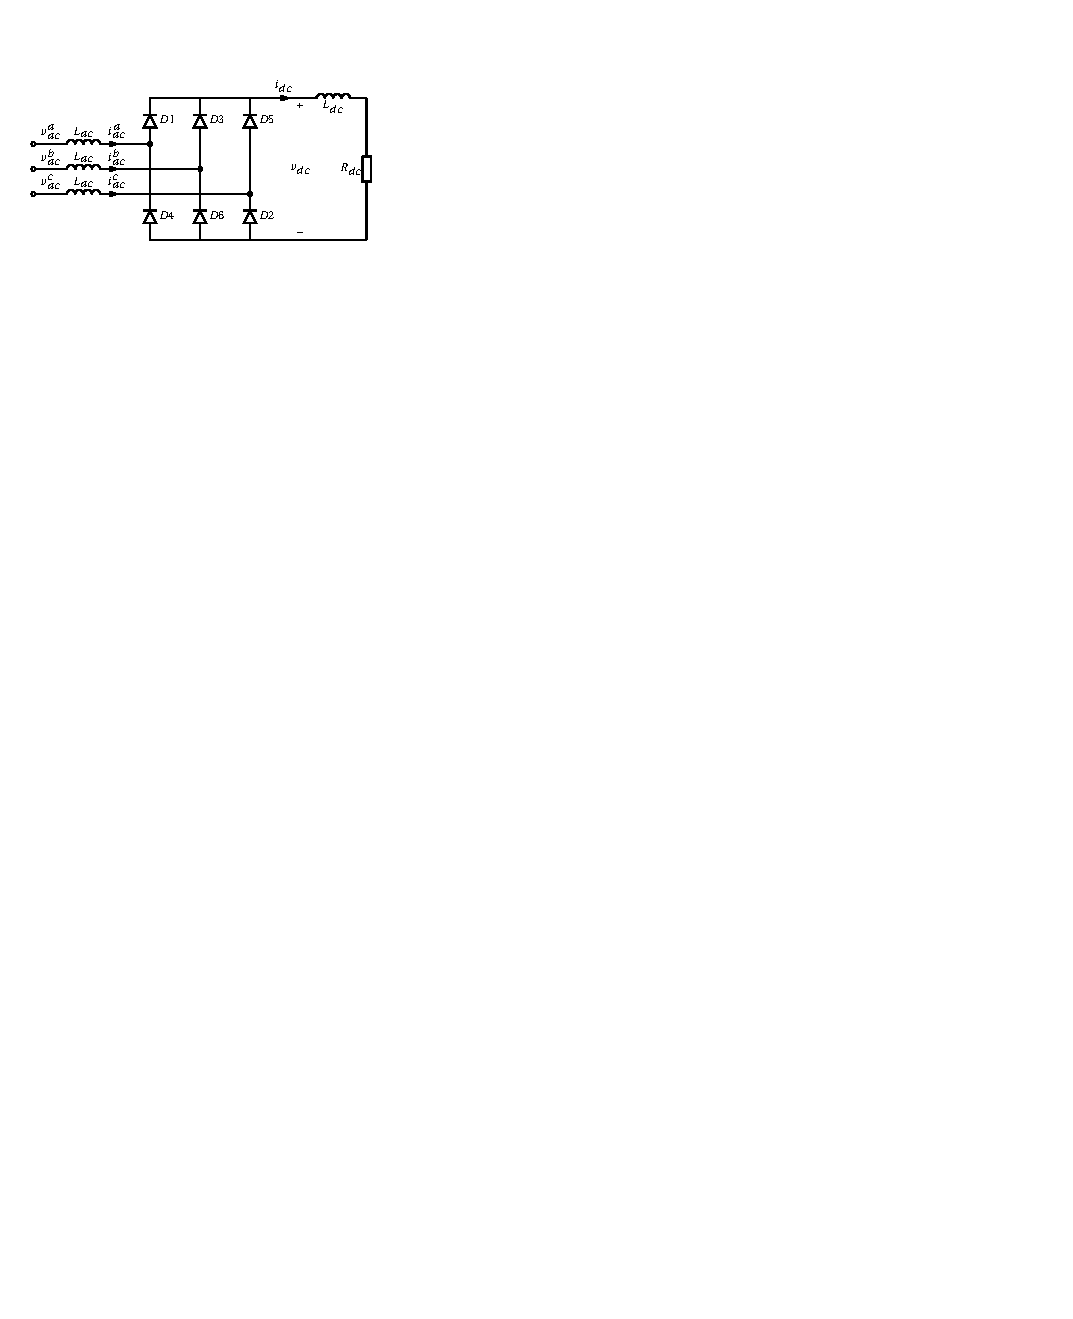
\includegraphics[width=0.6\columnwidth]{figures/topo_indust_LCC.pdf}
\caption{6-pulse line-commutated converter with ac-side commutation inductance~$L_{ac}$, dc-side smoothing inductance~$L_{dc}$ and dc load.}
\label{fig:topo_indust_LCC} 
\end{figure}

\subsection{Steady-State Harmonic Model} 
% Internal frequency coupling is the key feature of converter-generated harmonics, which decide the recombination of harmonic phasors. Therefore, the accurate harmonic state-space model is built here to capture the nature commutation and harmonic coupling of line-commutated converter.

The steady-state harmonic state-space model is used here to accurately capture the nature commutation and internal harmonic coupling of the line-commutated converter. The line-commutated converter periodically operates with sequential switching states, including 6 conducting states and 6 commutation states per fundamental period. Each state can be described by differential equations with time-varying coefficients that represent topology variations. The state equations for any switching state can be expressed as,
\begin{IEEEeqnarray}{l}
    (S_{dc} L_{ac} + L_{dc}) \frac{di_{dc}}{dt} = \nonumber \\
    S_{dc,ac}^{a} v_{ac}^a + S_{dc,ac}^{b} v_{ac}^b + S_{dc,ac}^{c} v_{ac}^c - R_{dc} i_{dc}, \label{eq:idc_t} \\
    % L_{ac} \frac{di_{ac}^a}{dt} - S_{dc,ac}^{a} L_{ac} \frac{di_{dc}}{dt} = \nonumber \\ S_{ac}^{a,a} v_{ac}^a + S_{ac}^{a,b} v_{ac}^b + S_{ac}^{a,c} v_{ac}^c, \label{eq:iac_t} \\
    L_{ac} \frac{di_{ac}^i}{dt} - S_{dc,ac}^{i} L_{ac} \frac{di_{dc}}{dt} = \nonumber \\ S_{ac}^{i,a} v_{ac}^a + S_{ac}^{i,b} v_{ac}^b + S_{ac}^{i,c} v_{ac}^c, \label{eq:iac_t}
\end{IEEEeqnarray}
where $v_{ac}^{i}$ and $i_{ac}^{i}$ denote ac-side voltage and current, $v_{dc}$ and $i_{dc}$ are dc-side voltage and current, the superscript $i,j \in \{a, b, c\}$ represents the three phases, $S_{dc,ac}^{i}(t)$, $S_{dc}(t)$, and $S_{ac}^{i,j}(t)$ are the piecewise switching functions reflecting the topology states.

The periodic equations in time-domain can be transformed into the harmonic state-space model in harmonic-domain through three operations: (i) Fourier series expansion of state variables $x(t) \leftrightarrow \sum_{h=-N_h}^{N_h} X_h e^{jh\omega_1 t}$ with truncated order $N_h$, (ii) frequency-domain differentiation $dx/dt \leftrightarrow \mathbf{Z}_{\Omega}\mathbf{X}$ where $\mathbf{Z}_{\Omega} = j\omega_1 \cdot \text{diag}(h)$, and (iii) Toeplitz convolution matrices representing time-domain multiplication: $y(t) = S(t)x(t) \leftrightarrow \mathbf{Y} = \mathbf{S}_{conv}\mathbf{X}$. The resulting unified system relates current harmonics $\mathbf{I} = [\mathbf{I}_{ac}^a, \mathbf{I}_{ac}^b, \mathbf{I}_{ac}^c]^T$ to voltage harmonics $\mathbf{U} = [\mathbf{V}_{ac}^a, \mathbf{V}_{ac}^b, \mathbf{V}_{ac}^c]^T$ through:

\begin{equation}
\mathbf{A}\mathbf{I} = \mathbf{B}\mathbf{U},
\label{eq:HSS}
\end{equation}
where matrices $\mathbf{A}$ and $\mathbf{B}$ contain Toeplitz convolution structures that explicitly capture frequency coupling. The model is parameterized by commutation overlap angle $\mu$, and the circuit inductances ($L_{ac}$, $L_{dc}$), providing a foundation for subsequent Monte Carlo simulation and uncertainty quantification.

\subsection{Methodology for Uncertainty Quantification}
In the planning stage, the uncertainty on key parameters comes from limited knowledge about the future integrated device, as well as manufacturing tolerances and operational variances. Therefore, inductance parameters $L_{ac}$ and $L_{dc}$ are modeled as random variables, and Monte Carlo simulation is used to assess the propagation of uncertainty.

\subsubsection{Realistic Parameter Distribution}
The uncertainties on $L_{ac}$ and $L_{dc}$ are modeled using truncated normal distributions:
\begin{equation}
L_{ac} \sim \mathcal{N}_{\text{trunc}}(\mu_{L_{ac}}, \sigma_{L_{ac}}^2, L_{ac,\min}, L_{ac,\max})
\label{truncated_normal_lac}
\end{equation}
\begin{equation}
L_{dc} \sim \mathcal{N}_{\text{trunc}}(\mu_{L_{dc}}, \sigma_{L_{dc}}^2, L_{dc,\min}, L_{dc,\max})
\label{truncated_normal_ldc}
\end{equation}
which are constrained within physically realistic bounds determined by engineering trade-offs at the industrial load design stage. For ac inductance $L_{ac}$, the upper bound $L_{ac,\max}$ is limited by the acceptable commutation angle and voltage drop, while the lower bound $L_{ac,\min}$ ensures adequate harmonic suppression and safe short-circuit current. For dc inductance $L_{dc}$, the upper bound $L_{dc,\max}$ is limited by dynamic response and size, while the lower bound $L_{dc,\min}$ ensures dc ripple to be within the specifications of power quality. The truncated normal distribution enforces physical bounds while maintaining mathematical tractability for Monte Carlo propagation.

% \begin{itemize}
%     \item \textit{ac-side inductance $L_{ac}$:} The upper bound $L_{ac,\max}$ is limited by acceptable commutation angle and voltage drop, while the lower bound $L_{ac,\min}$ ensures adequate harmonic suppression and safe short-circuit current.
%     \item \textit{dc-side inductance $L_{dc}$:} The upper bound $L_{dc,\max}$ is limited by required dynamic response, size, and cost, while the lower bound $L_{dc,\min}$ ensures dc ripple stays within specifications to prevent equipment aging and process quality degradation.
% \end{itemize}

\subsubsection{Monte Carlo Simulation}
Monte Carlo simulation is then implemented, by which 5000 pairs of random samples $(L_{ac}, L_{dc})$ are generated using rejection sampling to meet the defined constraints. For each of the parameter samples, a harmonic state-space model is built and solved. The iterative process involves: (i) recalculating the commutation angle $\mathsf{\mu}$ based on the sample pair of parameters; (ii) reconstructing the time-periodic switching functions $S_{dc,ac}^{i}(t)$, $S_{dc}(t)$, and $S_{ac}^{i,j}(t)$ using the updated commutation angle; and (iii) numerically solving the harmonic state-space equations to extract and store the magnitudes and phase angles of the ac-side harmonics.
% \begin{itemize}
%     \item Recalculating the commutation angle $\mathsf{\mu}$ based on the sampled pair of parameters.
%     \item Reconstructing time-periodic switching functions $S_{dc,ac}^{i}(t)$, $S_{dc}(t)$, and $S_{ac}^{i,j}(t)$ based on the updated commutation angle.
%     % \item Reconstructing time-periodic switching functions $\mathbf{S}_{dc,ac,conv}^{i}$, $\mathbf{S}_{dc,conv}$, and $\mathbf{S}_{ac,conv}^{i,j}$ based on the updated commutation angle.
%     \item Numerically solving the harmonic state-space equations to extract and store the magnitudes and phase angles of the ac-side harmonic currents of interest.
% \end{itemize}

\subsection{Dependency Analysis and Probability Density Function}
A case study is conducted based on a representative 6-pulse line-commutated converter unit, with nominal capacity of 1.25 MW and nominal voltage of 380 V, which is connected to the 35 kV bus through a rectifier transformer with a ratio of 35 kV/400 V. 
For the ac-side commutation inductance, the truncation bounds are $L_{ac,\min} = 0.01$ mH and $L_{ac,\max} = 0.03$ mH, corresponding to transformer short-circuit voltage ranging from $U_k = 5\%$ to $15\%$. For the dc-side smoothing inductance, the truncation bounds are $L_{dc,\min} = 0.05$ mH and $L_{dc,\max} = 0.35$ mH.

Fig.\ref{fig:harmonic_phasors_CI_LacLdc} shows the resulting phasor distribution of each characteristic harmonic. In each harmonic phasor distribution plot, the black arrow represent the phasors with mean magnitude and mean phase angle, while the dark gray represent the phasors within the 95\% confidence intervals. The results indicate that (i) the harmonic phasors at different frequencies exhibit mutual dependency; (ii) harmonics at higher orders display progressively larger angle variations and uncertainties. 

% \begin{figure}[!t]
%     \centering
%     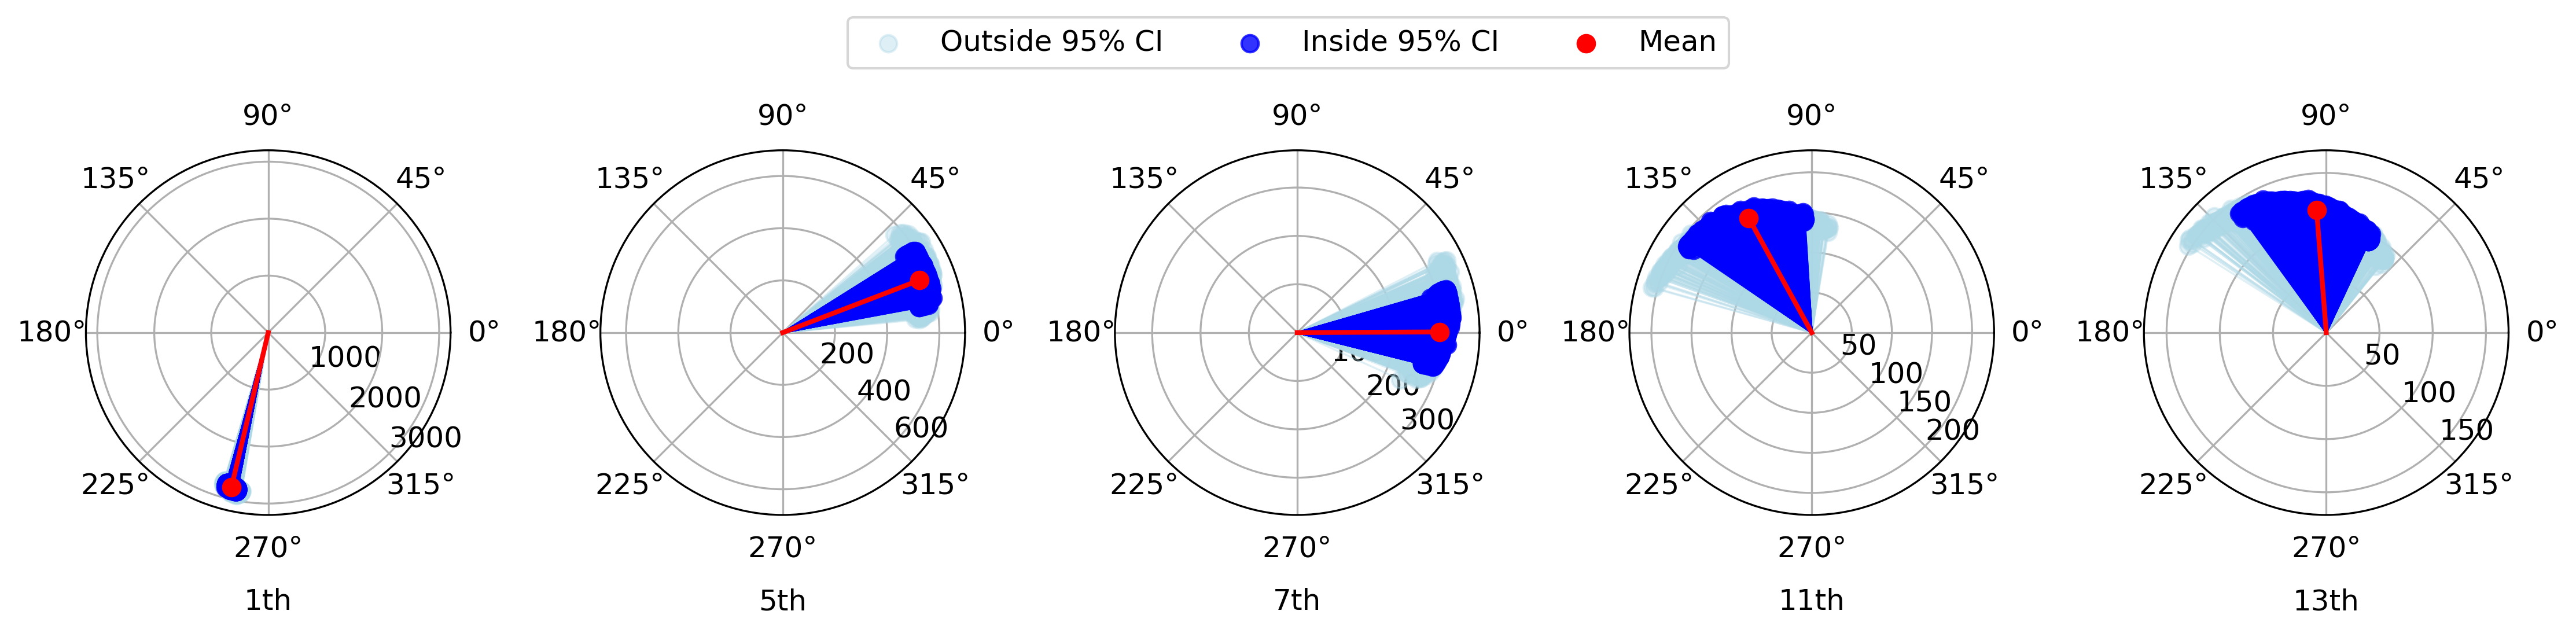
\includegraphics[width=\columnwidth]{figures/harmonic_phasors_CI_LacLdc.png}
%     \caption{Phasors of the characteristic harmonic currents of the converter of Fig.~\ref{fig:topo_indust_LCC} for 5000 Monte Carlo samples of~$L_{ac}$ and~$L_{dc}$: phasor with the mean magnitude and mean phase angle (red) and phasors within the 95\,\% confidence intervals (blue).}
%     \label{fig:harmonic_phasors_CI_LacLdc}
% \end{figure}

\usepgfplotslibrary{polar}
\providecommand{\Harmonic}{h}
\begin{figure*}[!t]
    \centering
    \pgfplotsset{phasorplot/.style={shhc, width=0.18\textwidth, ymin=0,
        xtick={0,90,180,270}, xticklabel={$\pgfmathprintnumber{\tick}^{\circ}$},
        yticklabel style={font=\tiny, anchor=north, inner sep=1.5pt, yshift=-2pt, /pgf/number format/1000 sep={}},
        every axis plot/.append style={line join=round}},
        outside/.style={only marks, mark=*, mark size=0.5pt, gray!35},
        inside/.style={only marks, mark=*, mark size=0.5pt, black!70},
        ci/.style={densely dashed, black, line width=0.5pt, mark=none},
        meanphasor/.style={-latex, black, line width=1pt, mark=none}}
    \subfloat[$\Harmonic = 1$]{%
    \begin{tikzpicture}
        \begin{polaraxis}[phasorplot, ymax=3200, ytick={1000,2000}, yticklabels={1k,2k}]
            \addplot[outside] table[x=angle, y=mag] {journals/shhc/data/phasor_ci/plot_outside_h1.dat};
            \addplot[inside] table[x=angle, y=mag] {journals/shhc/data/phasor_ci/plot_inside_h1.dat};
            \addplot[ci] table[x=angle, y=mag] {journals/shhc/data/phasor_ci/ci_h1.dat};
            \addplot[meanphasor] table[x=angle, y=mag] {journals/shhc/data/phasor_ci/mean_h1.dat};
        \end{polaraxis}
    \end{tikzpicture}}%
    \subfloat[$\Harmonic = 5$]{%
    \begin{tikzpicture}
        \begin{polaraxis}[phasorplot, ymax=700, ytick={300,600}]
            \addplot[outside] table[x=angle, y=mag] {journals/shhc/data/phasor_ci/plot_outside_h5.dat};
            \addplot[inside] table[x=angle, y=mag] {journals/shhc/data/phasor_ci/plot_inside_h5.dat};
            \addplot[ci] table[x=angle, y=mag] {journals/shhc/data/phasor_ci/ci_h5.dat};
            \addplot[meanphasor] table[x=angle, y=mag] {journals/shhc/data/phasor_ci/mean_h5.dat};
        \end{polaraxis}
    \end{tikzpicture}}%
    \subfloat[$\Harmonic = 7$]{%
    \begin{tikzpicture}
        \begin{polaraxis}[phasorplot, ymax=370, ytick={150,300}, yticklabels={150,}]
            \addplot[outside] table[x=angle, y=mag] {journals/shhc/data/phasor_ci/plot_outside_h7.dat};
            \addplot[inside] table[x=angle, y=mag] {journals/shhc/data/phasor_ci/plot_inside_h7.dat};
            \addplot[ci] table[x=angle, y=mag] {journals/shhc/data/phasor_ci/ci_h7.dat};
            \addplot[meanphasor] table[x=angle, y=mag] {journals/shhc/data/phasor_ci/mean_h7.dat};
        \end{polaraxis}
    \end{tikzpicture}}%
    \subfloat[$\Harmonic = 11$]{%
    \begin{tikzpicture}
        \begin{polaraxis}[phasorplot, ymax=230, ytick={100,200}]
            \addplot[outside] table[x=angle, y=mag] {journals/shhc/data/phasor_ci/plot_outside_h11.dat};
            \addplot[inside] table[x=angle, y=mag] {journals/shhc/data/phasor_ci/plot_inside_h11.dat};
            \addplot[ci] table[x=angle, y=mag] {journals/shhc/data/phasor_ci/ci_h11.dat};
            \addplot[meanphasor] table[x=angle, y=mag] {journals/shhc/data/phasor_ci/mean_h11.dat};
        \end{polaraxis}
    \end{tikzpicture}}%
    \subfloat[$\Harmonic = 13$]{%
    \begin{tikzpicture}
        \begin{polaraxis}[phasorplot, ymax=170, ytick={50,100}]
            \addplot[outside] table[x=angle, y=mag] {journals/shhc/data/phasor_ci/plot_outside_h13.dat};
            \addplot[inside] table[x=angle, y=mag] {journals/shhc/data/phasor_ci/plot_inside_h13.dat};
            \addplot[ci] table[x=angle, y=mag] {journals/shhc/data/phasor_ci/ci_h13.dat};
            \addplot[meanphasor] table[x=angle, y=mag] {journals/shhc/data/phasor_ci/mean_h13.dat};
        \end{polaraxis}
    \end{tikzpicture}}
    \caption{Phasors of characteristic harmonic currents, 1000 of the 5000 Monte Carlo samples, inside (dark gray) and outside (light gray) the 95\,\% confidence region of magnitude and phase angle (dashed), with the mean phasor (black arrow): (a) $\Harmonic = 1$; (b) $\Harmonic = 5$; (c) $\Harmonic = 7$; (d) $\Harmonic = 11$; (e) $\Harmonic = 13$.}
    \label{fig:harmonic_phasors_CI_LacLdc}
\end{figure*}

\subsubsection{Inter-Harmonic Dependency Analysis}
An important feature of the harmonics generated by the line-commutated converter is the inter-harmonic dependency due to frequency coupling, as indicated by the harmonic state-space model in ~\eqref{eq:HSS}. To characterize the dependencies among harmonic components, the correlation matrices with Kendall's Tau correlation coefficients are obtained.
% To assess this dependency, the correlation structure between different harmonic components is investigated. Correlation matrices, with Kendall's Tau correlation coefficients, are used to characterize the dependencies.
As shown by the phase angle correlation matrix $\mathbf{R}_{\text{phase}}$ in Fig.~\ref{fig:Correlation_Matrix_Copula}, phase angles have strong inter-harmonic dependency with the Gaussian copula parameters $\rho_{ij}^{Gauss} \geq 0.97$.
% indicating distinct characteristics in the inter-harmonic dependency structure for phase angles.

% \begin{figure}[!t]
%     \centering
%     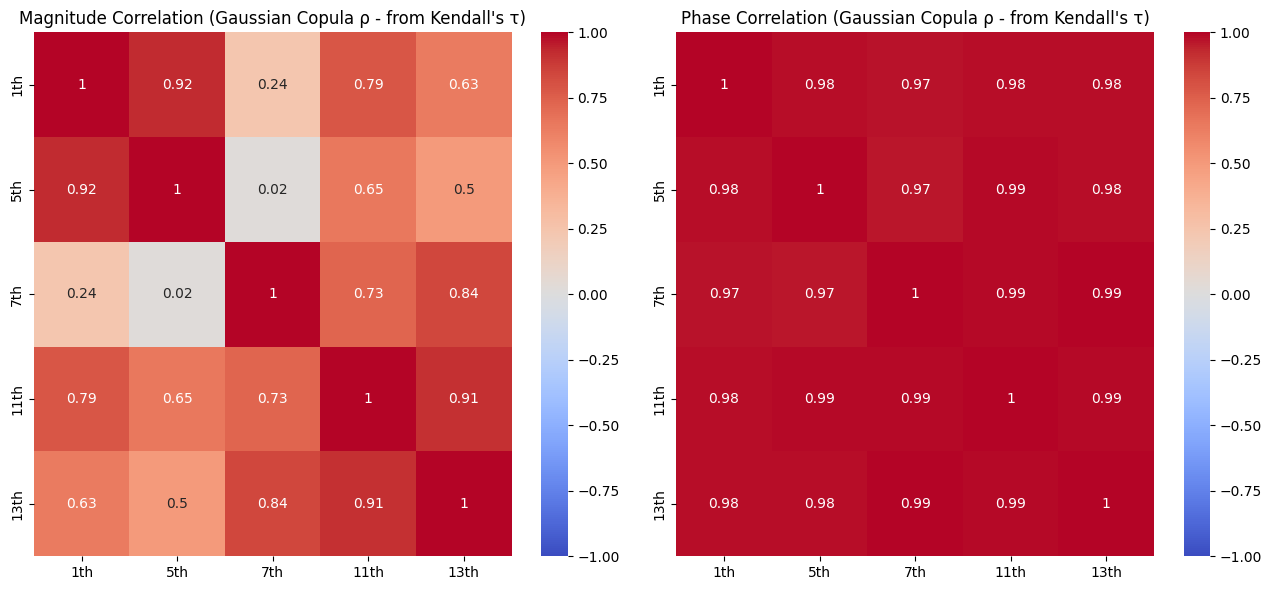
\includegraphics[width=\columnwidth]{figures/Correlation_Matrix_Copula.png}
%     \caption{Gaussian copula correlation matrices of the harmonic current magnitudes and of the harmonic current phase angles across the harmonic orders, from 5000 Monte Carlo samples of~$L_{ac}$ and~$L_{dc}$.}
%     \label{fig:Correlation_Matrix_Copula}
% \end{figure}

\providecommand{\Harmonic}{h}
\begin{figure}[!t]
    \centering
    \pgfplotsset{corrplot/.style={shhc, grid=none, scale only axis, width=3.2cm, height=3.2cm,
        xmin=-0.5, xmax=4.5, ymin=-0.5, ymax=4.5, y dir=reverse, axis on top,
        xtick={0,...,4}, ytick={0,...,4}, xticklabels={1,5,7,11,13}, yticklabels={1,5,7,11,13},
        tick style={draw=none}, xlabel={harmonic order $\Harmonic$},
        colormap={gray}{color=(white) color=(gray!70)}, point meta min=0, point meta max=1,
        nodes near coords={\pgfmathprintnumber[fixed, fixed zerofill, precision=2]{\pgfplotspointmeta}},
        every node near coord/.append style={font=\tiny, black, anchor=center}},
        corrcells/.style={matrix plot*, mesh/cols=5, point meta=explicit, draw=white, line width=0.4pt}}
    \subfloat[magnitude]{%
    \begin{tikzpicture}
        \begin{axis}[corrplot, ylabel={harmonic order $\Harmonic$}]
            \addplot[corrcells] table[x=col, y=row, meta=rho] {journals/shhc/data/copula_corr/corr_mag.dat};
        \end{axis}
    \end{tikzpicture}}%
    \subfloat[phase angle]{%
    \begin{tikzpicture}
        \begin{axis}[corrplot]
            \addplot[corrcells] table[x=col, y=row, meta=rho] {journals/shhc/data/copula_corr/corr_phase.dat};
        \end{axis}
    \end{tikzpicture}}
    \caption{Dependence between the harmonic currents of the industrial load, Gaussian copula correlation matrices with parameters $\rho_{ij}^{Gauss}$ obtained from Kendall's rank correlation~$\tau$ of 5000 Monte Carlo samples, darker cells for stronger correlation: (a) magnitudes; (b) phase angles.}
    \label{fig:Correlation_Matrix_Copula}
\end{figure}

% \subsubsection{Marginal Distribution Fitting}
% The marginal distributions of each harmonic component are modeled independently. The best-fit probability density function for each harmonic magnitude and phase angle is fitted to the data obtained from Monte Carlo simulation. The candidate distributions considered include Normal, Lognormal, Beta, Logistic and Exponential distributions.

% For each harmonic $h$, the marginal distribution $F_h(x_h)$ is estimated by fitting multiple parametric distributions and selecting the best-fit  distribution based on minimizing the root-mean-square error between the cumulative distribution functions simulated and fitted. The best-fit results are illustrated in Fig.\ref{fig:Bestfit_PDF}, showing the histograms and the fitted probability density functions of harmonic magnitudes and phase angles.

% Tables~\ref{tab:bestfit_phase} summarize the best-fit distributions and their estimated parameters for harmonic phase angles.
% \begin{table}[h] 
% \centering
% \caption{Best-Fit Distributions for Harmonic Phase Angles}
% \label{tab:bestfit_phase}
% \begin{tabular}{l l l l}
% \hline
% Order & distribution & error & parameters \\
% \hline
% 1st  & Beta    & $9.30 e^{-3}$ & $[ 10.8052, 20.2376, -107.9443, 13.0245]$ \\
% 5th  & Beta    & $1.97 e^{-3}$ & $[11.8144, 23.6725, -2.6825, 70.8689]$ \\
% 7th  & Beta    & $1.54 e^{-3}$ & $[ 9.7918, 18.8775, -29.9737, 88.2789]$ \\
% 11th & Beta    & $7.41 e^{-4}$ & $[ 12.4463, 22.1493, 59.5585, 164.3101]$ \\
% 13th & Beta    & $6.84 e^{-4}$ & $[ 10.4088, 17.2887, 29.4667, 172.4882]$ \\
% \hline
% \end{tabular}
% \end{table}

% The parameters of the Beta distribution are given as $[\alpha, \beta, \ell, \theta]$, where $\alpha$ and $\beta$ are the shape parameters, and $\ell$ and $\theta$ are the location and scale parameters, respectively.

% \begin{figure*}[h!]
%     \centering
%     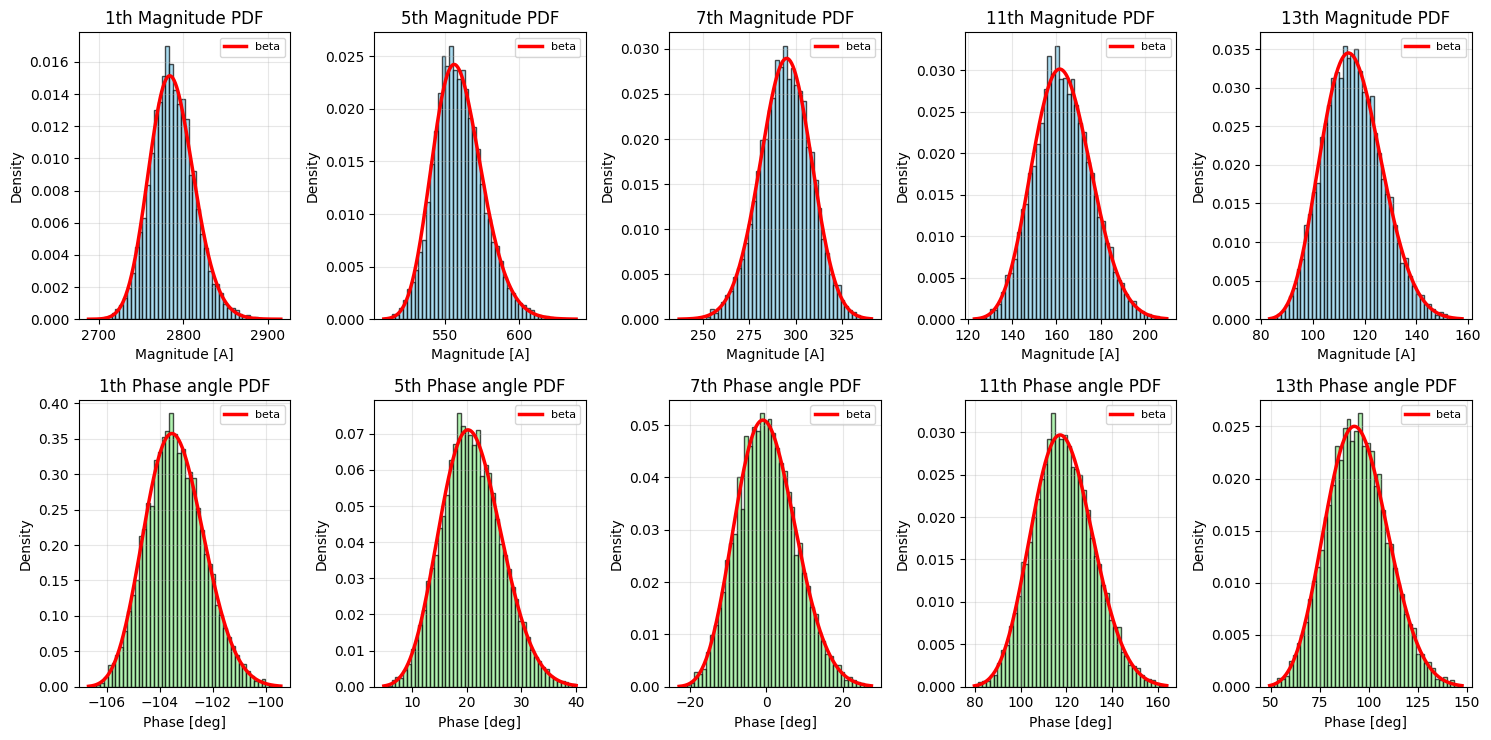
\includegraphics[width=0.8\textwidth]{figures/Bestfit_PDF.png}
%     \caption{Histograms of the harmonic current magnitudes and phase angles from 5000 Monte Carlo samples of~$L_{ac}$ and~$L_{dc}$, with the best-fit probability density functions of Table~\ref{tab:bestfit_phase}.}
%     \label{fig:Bestfit_PDF} 
% \end{figure*}

\subsubsection{Shared Beta Distribution for Phase Angles}
Since strong inter-harmonic dependencies are proved for phase angles, a shared Beta distribution is used to represent the normalized phase angle distributions across the harmonic orders. In this way, only two shape parameters, $\alpha$ and $\beta$, are estimated for all harmonics, while each harmonic retains its own location and scale parameters to capture the specific range of phase angles.

Firstly, a normalization procedure is applied to the unwrapped phase angle data of each harmonic to map them to the unit interval $[0,1]$. Let $\phi_h = \{\phi_{h,i}\}_{i=1}^{N}$ denote the unwrapped phase angle samples in degrees for harmonic $h \in \{1, 5, 7, 11, 13\}$, where unwrapping avoids discontinuities at $\pm 180^\circ$. For each harmonic, the observed min–max values are $v_{\min,h} = \min(\phi_h)$ and $v_{\max,h} = \max(\phi_h)$.
% \begin{equation}
% v_{\min,h} = \min(\phi_h), \qquad v_{\max,h} = \max(\phi_h).
% \end{equation}
The sampled data of each harmonic phase angle are then normalized to the unit interval via the min-max transformation:
\begin{equation}
u_{h,i} = \frac{\phi_{h,i} - v_{\min,h}}{v_{\max,h} - v_{\min,h}} \in (0,1).
\end{equation}

Secondly, all normalized samples from the five harmonics are pooled into a single dataset:
\begin{equation}
\mathcal{U} = \bigcup_{h \in \{1,5,7,11,13\}} \{u_{h,i}\}_{i=1}^{N}.
\end{equation}

A single Beta distribution with estimated shape parameters $\hat{\alpha}$ and $\hat{\beta}$ is fitted to $\mathcal{U}$ via maximum likelihood estimation, with location and scale fixed to the standard interval $[0,1]$:
\begin{equation}
u \sim \mathrm{Beta}(\hat{\alpha}, \hat{\beta}).
\end{equation}

The results of the fitted parameters are $\hat{\alpha} = 4.0414$, $\hat{\beta} = 4.7762$. The Beta probability density function is given by:
\begin{equation}
f_{\mathrm{Beta}}(u; \hat{\alpha}, \hat{\beta}) = \frac{u^{\hat{\alpha}-1}(1-u)^{\hat{\beta}-1}}{\int_0^1 t^{\hat{\alpha}-1}(1-t)^{\hat{\beta}-1}\,dt}, \quad u \in (0,1).
\end{equation}

Thirdly, the fitted shared Beta distribution is transformed back to each harmonic's phase angle scale to assess the goodness-of-fit. For each harmonic $h$, the denormalization is performed as:
\begin{equation}
\label{eq:beta_denorm}
f_{\phi_h}(\phi) = \frac{1}{v_{\max,h} - v_{\min,h}} \, f_{\mathrm{Beta}}\!\left(\frac{\phi - v_{\min,h}}{v_{\max,h} - v_{\min,h}}; \hat{\alpha}, \hat{\beta}\right),
\end{equation}
where $\phi\in [v_{\min,h}, v_{\max,h}]$ is the original phase angle range for harmonic $h$.

Table~\ref{tab:beta_phase_params} lists the shared shape parameters, harmonic-specific locations $v_{\min,h}$ and scales $(v_{\max,h} - v_{\min,h})$, and the root-mean-square errors between the empirical histograms from the Monte Carlo simulation and the denormalized Beta probability density functions.
% The goodness-of-fit of the shared Beta distribution model is evaluated for each harmonic phase angle by comparing the denormalized Beta probability density function against the empirical histograms from Monte Carlo simulation. The root-mean-square error is computed between the empirical histogram and the denormalized Beta probability density function, with the results summarized in last column of Table~\ref{tab:beta_phase_params}.
The comparison plots between the empirical histograms and the denormalized shared Beta probability density functions for each harmonic phase angle are shown in Fig.~\ref{fig:Shared_Beta_Fit}. Both the visual comparison and the low root-mean-square errors indicate a good fit of the shared Beta distribution to the simulated data across all harmonics.

\begin{table}[!t]
    \centering
    \caption{Shared Beta distribution parameters and fit quality for harmonic phase angles}
    \label{tab:beta_phase_params}
    \scriptsize
    \begin{tabular}{l c c c c}
    Order & $v_{\min}$ [deg] & $v_{\max}$ [deg] & $v_{\max} - v_{\min}$ [deg] & error \\
    \hline
    1st  & $-106.70$ & $-99.43$   & 7.27   & 0.0226 \\
    5th  & 4.75      & 40.05      & 35.30  & 0.0037 \\
    7th  & $-22.77$  & 27.51      & 50.28  & 0.0029 \\
    11th & 79.69     & 164.01     & 84.32  & 0.0014 \\
    13th & 49.38     & 147.67     & 98.29  & 0.0011 \\
    \end{tabular}
    
    \vspace{2pt}
    \parbox{\columnwidth}{\scriptsize All harmonics share the same shape parameters ($\hat{\alpha} = 4.041$, $\hat{\beta} = 4.776$).\\
    Location parameters $v_{\min}$ and scale parameter $(v_{\max} - v_{\min})$ are harmonic-specific.}
    % \multicolumn{7}{l}{\footnotesize Note: All harmonics share the same shape parameters ($\hat{\alpha} = 4.041$, $\hat{\beta} = 4.776$).} \\
    % \multicolumn{7}{l}{\footnotesize Location parameter $v_{\min}$ and scale parameter $(v_{\max} - v_{\min})$ are harmonic-specific.} \\
\end{table}

% \begin{figure}[!b]
%     \centering
%     % 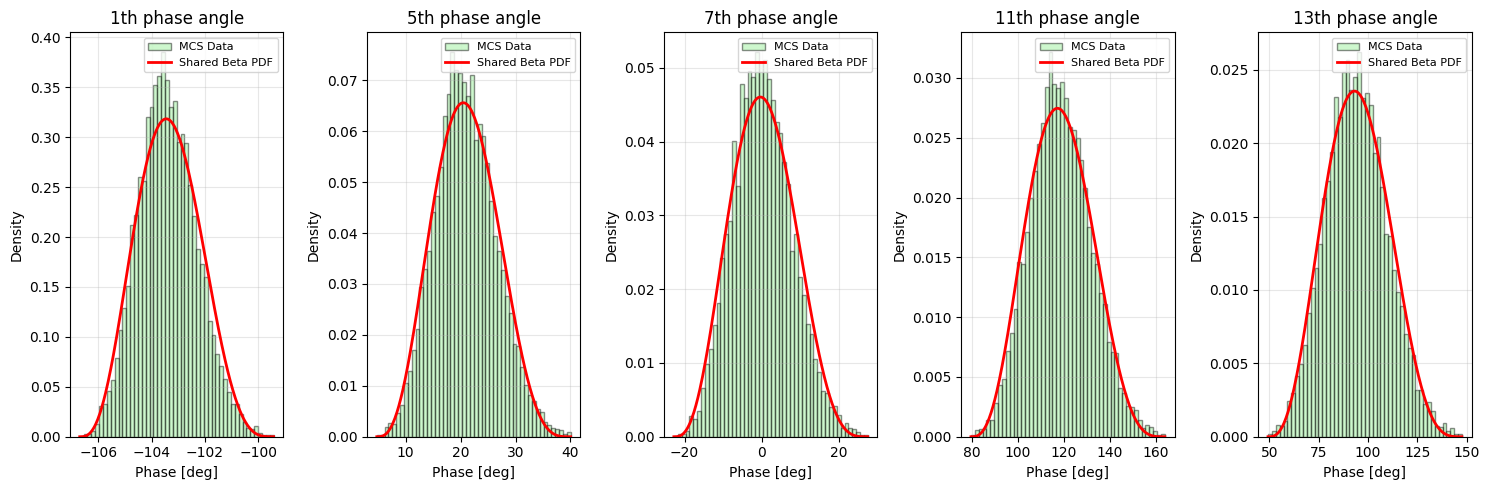
\includegraphics[width=0.8\textwidth]{figures/Shared_Beta_Fit.png}
%     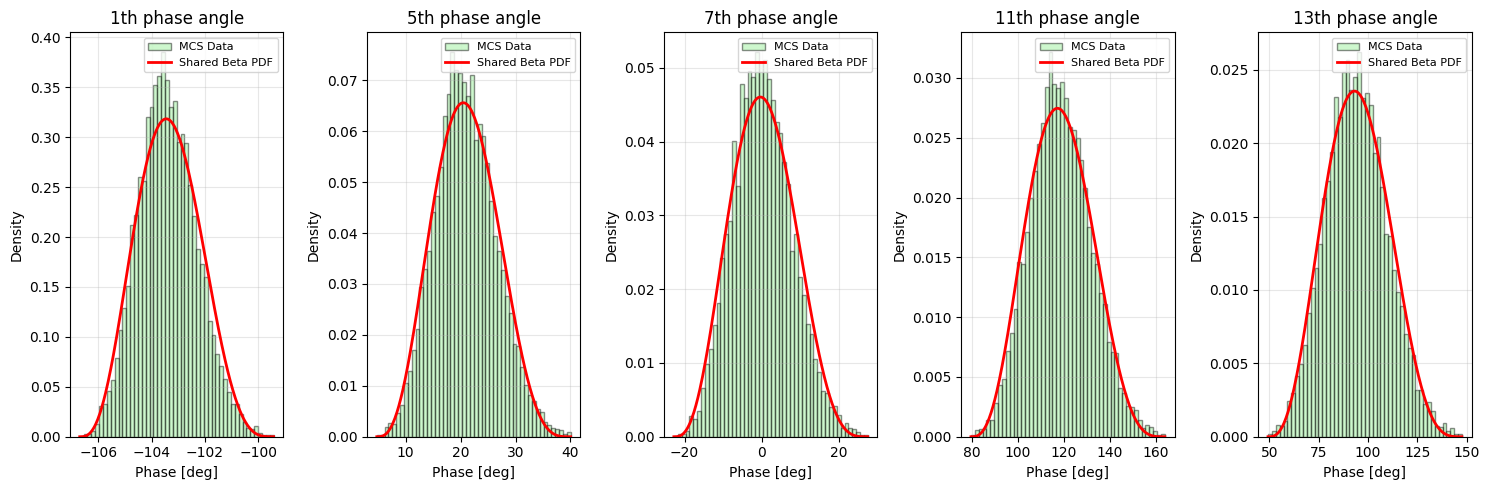
\includegraphics[width=\columnwidth]{figures/Shared_Beta_Fit.png}
%     \caption{Histograms of the harmonic current phase angles from 5000 Monte Carlo samples of~$L_{ac}$ and~$L_{dc}$, and the denormalized shared Beta probability density functions with parameters listed in Table~\ref{tab:beta_phase_params}.}
%     \label{fig:Shared_Beta_Fit} 
% \end{figure}

\begin{figure*}[!t]
    \centering
    \pgfplotsset{phaseplot/.style={shhc, width=0.205\textwidth, height=3cm, ymin=0,
        xlabel={phase [deg]}, scaled y ticks=false, yticklabel style={/pgf/number format/fixed},
        every axis plot/.append style={mark=none}},
        mcs/.style={ybar interval, fill=gray!30, draw=gray!70, line width=0.2pt},
        beta/.style={solid, black, line width=0.9pt}}
    \subfloat[$h = 1$]{%
    \begin{tikzpicture}
        \begin{axis}[phaseplot, xtick={-106,-103,-100}, ylabel={PDF [1/deg]}]
            \addplot[mcs] table[x=x, y=density] {journals/shhc/data/shared_beta_phase/hist_interval_h1.dat};
            \addplot[beta] table[x=x, y=pdf] {journals/shhc/data/shared_beta_phase/pdf_h1.dat};
        \end{axis}
    \end{tikzpicture}}%
    \subfloat[$h = 5$]{%
    \begin{tikzpicture}
        \begin{axis}[phaseplot, xtick={10,20,30}]
            \addplot[mcs] table[x=x, y=density] {journals/shhc/data/shared_beta_phase/hist_interval_h5.dat};
            \addplot[beta] table[x=x, y=pdf] {journals/shhc/data/shared_beta_phase/pdf_h5.dat};
        \end{axis}
    \end{tikzpicture}}%
    \subfloat[$h = 7$]{%
    \begin{tikzpicture}
        \begin{axis}[phaseplot, xtick={-20,0,20}]
            \addplot[mcs] table[x=x, y=density] {journals/shhc/data/shared_beta_phase/hist_interval_h7.dat};
            \addplot[beta] table[x=x, y=pdf] {journals/shhc/data/shared_beta_phase/pdf_h7.dat};
        \end{axis}
    \end{tikzpicture}}%
    \subfloat[$h = 11$]{%
    \begin{tikzpicture}
        \begin{axis}[phaseplot, xtick={90,120,150}]
            \addplot[mcs] table[x=x, y=density] {journals/shhc/data/shared_beta_phase/hist_interval_h11.dat};
            \addplot[beta] table[x=x, y=pdf] {journals/shhc/data/shared_beta_phase/pdf_h11.dat};
        \end{axis}
    \end{tikzpicture}}%
    \subfloat[$h = 13$]{%
    \begin{tikzpicture}
        \begin{axis}[phaseplot, xtick={60,100,140}]
            \addplot[mcs] table[x=x, y=density] {journals/shhc/data/shared_beta_phase/hist_interval_h13.dat};
            \addplot[beta] table[x=x, y=pdf] {journals/shhc/data/shared_beta_phase/pdf_h13.dat};
        \end{axis}
    \end{tikzpicture}}
    \caption{Distribution of harmonic current phase angles, histograms of 5000 Monte Carlo samples (gray, 50 bins) against the denormalized shared Beta probability density functions (balck) with parameters listed in Table~\ref{tab:beta_phase_params}: (a) $h = 1$; (b) $h = 5$; (c) $h = 7$; (d) $h = 11$; (e) $h = 13$.}
    \label{fig:Shared_Beta_Fit}
\end{figure*}


\subsection{Second Converter Type: Phase-Controlled Rectifier}
\label{sec:converter_types}

The analysis above concerns a single converter type. Real networks host a mix of converter technologies, whose harmonic current angles differ in their mean. As a second type, a phase-controlled version of the same 6-pulse converter is considered, i.e., a thyristor rectifier operated at a firing delay~$\alpha_{\text{f}}$. Delaying the firing delays the whole current waveform, which rotates the $h$-th harmonic phasor of phase~$a$ by~$-h\,\alpha_{\text{f}}$ relative to the uncontrolled converter, while the dispersion caused by the uncertain inductances is retained. The firing delay is set by the operating point, e.g., the demanded dc voltage, and is therefore common to all units of this type and uncertain at the planning stage.

\emph{Working assumption.} Pending a dedicated harmonic state-space analysis of the phase-controlled converter, the firing delay is modelled with a mean of~$30^{\circ}$ and a Beta-distributed support of~$30^{\circ}$ width, with the shape parameters of Table~\ref{tab:beta_phase_params}, and the overlap angle is assumed independent of the firing delay. The resulting angle model, with one germ shared by all units of the type, is given in Section~\ref{sec:harmonic_current_angle_uncertainty}.


\section{Mathematical Framework}
\label{sec:mathematical_framework}

This section presents the mathematical framework for the stochastic harmonic hosting capacity problem of a phase-balanced three-phase power system, considering uncertainty on the angle of the harmonic current injected by the connected harmonic units. To this end, the formulation for the deterministic harmonic hosting capacity presented in~\cite{vanacker_dhhc} is extended. For brevity, the original formulation is not repeated in this section, rather the relevant variables and constraints are highlighted and transformed to their stochastic counterpart.

First, Section~\ref{sec:polynomial_chaos_expansion} introduces the generalized polynomial chaos expansion method used to incorporate random variables into the formulation. Second, Section~\ref{sec:harmonic_current_angle_uncertainty} introduces the uncertainty on the angle of the injected harmonic current and a method to approximate the related trigonometric functions in the context of polynomial chaos expansion. Third, Section~\ref{sec:stochastic_harmonic_hosting_capacity} presents the transformation of the deterministic formulation into its stochastic counterpart and characterizes the resulting problem class. Finally, Section~\ref{sec:absolute_equality_lp} shows that for the absolute equality fairness criterion the problem reduces to an exact linear program. For the full stochastic formulation of the harmonic hosting capacity problem, the reader is referred to Appendix~\ref{app:optimization_model}.

In the following table, a general overview and generic examples of the notation used throughout the mathematical framework are provided.
\begin{table}[ht!]
    \centering
    \begin{tabular}{ l l c }
        element             & notation                  & example                           \\ \hline
        index               & lower-case italic         & $x$                               \\
        set                 & calligraphic              & $\mathcal{X}$                     \\
        (random) variable   & sans serif                & $\mathsf{X}$                      \\
        parameter           & italic                    & $X$                               \\
        approximation       & hat notation              & $\hat{\mathsf{X}}$                \\
        vector              & bar notation              & $\bar{\mathsf{X}}$, $\bar{X}$
    \end{tabular}
\end{table}

\subsection{Background on Polynomial Chaos Expansion}
\label{sec:polynomial_chaos_expansion}

This section introduces the necessary background on polynomial chaos expansion, a method for representing random variables in terms of polynomial functions. Concretely, a vector of input random variables, e.g., harmonic current angles, is propagated through the set of constraints of the harmonic hosting capacity problem to obtain a vector of unknown output random variables, e.g., harmonic bus voltages.

First, uncertainty quantification of random variables is introduced in terms of polynomial chaos expansion. Second and third, the impact of the polynomial chaos expansion method on equality and inequality constraints is discussed, respectively. For a detailed treatment of the subject, the reader is referred to~\cite{sullivan_introduction_2015}.

\subsubsection{Uncertainty Quantification}
In general, it is assumed that the stochastic input is captured by a real-valued finite-variance stochastic germ~$\bar{\omega} = [\omega_{1},...,\omega_{N}]^{\text{T}}$. Optimization solvers are unable to handle equations involving random variables directly, necessitating the formulation of a deterministic equivalent of the stochastic problem. For this purpose, polynomial chaos expansion approximates any real-valued random variable~$\RVX$ of finite variance that is a function of the stochastic germ~$\bar{\omega}$ as a linear combination~$\ApproxRVX$ of the orthogonal polynomial basis~$[\Polynoom_{\PCEIndex}(\bar{\omega})]_{\PCEIndex \in \PCESet}$, where $\PCESet\subseteq\NaturalNumberSet_{0}$, as,
\begin{IEEEeqnarray}{ r C l }
    \ApproxRVX &=& \sum_{\PCEIndex \in \PCESet} \CoefficientX_{\PCEIndex} \cdot \Polynoom_{\PCEIndex} =
    \sum_{\PCEIndex \in \PCESet} \frac{\langle \RVX, \Polynoom_{\PCEIndex} \rangle}{\langle \Polynoom_{\PCEIndex}, \Polynoom_{\PCEIndex} \rangle} \cdot \Polynoom_{\PCEIndex}, \label{eq:gpc_expansion}
\end{IEEEeqnarray}
where~$\CoefficientX_{\PCEIndex} \in \RealNumberSet$ denote the polynomial chaos expansion coefficients and $\langle \cdot,\cdot \rangle$ denotes the inner product. Through the use of the polynomial chaos expansion coefficients, a deterministic equivalent can be built for the stochastic problem. The choice of orthogonal polynomial basis depends on the distribution of the stochastic germ. In this work, following the Askey scheme~\cite{sullivan_introduction_2015}, Beta-distributed germ corresponds to Jacobi polynomials.

\subsubsection{Uncertainty Projection onto Equality Constraints}
An optimization problem requires an intrusive approach to exploit polynomial chaos expansion. Through polynomial chaos expansion, any stochastic equality constraint is equivalently represented by $|\PCESet|$ deterministic equality constraints. The total number of resulting equations, known as the cardinality of the model~$|\PCESet|$, is determined by the number of independent uncertainty sources and the highest polynomial degree as,
\begin{IEEEeqnarray}{ r C l }
    |\PCESet| &=& \frac{(|\bar{\omega}| + \delta)!}{|\bar{\omega}|!\,\delta!},
\end{IEEEeqnarray}
where~$\delta$ denotes the maximum degree of the polynomial basis functions. The truncation error~$\norm{\RVX-\ApproxRVX}$ decays to zero for~$|\PCESet| \to \infty$.

Additionally, the Galerkin projection is required to form a system of equations for the stochastic modes, which are generally coupled together~(Ch.~12 in~\cite{sullivan_introduction_2015}). For the purpose of the harmonic hosting capacity problem, in terms of the Galerkin projection, two distinct operations stand out: summation and multiplication. As an example, consider three approximated random variables~$\ApproxRVX$,~$\ApproxRVY$ and~$\ApproxRVZ$ defined using the same polynomial basis. The Galerkin projection (gp) of both operations is,
\begin{IEEEeqnarray}{ l C l l}
    \ApproxRVZ = \ApproxRVX + \ApproxRVY &\gp& \CoefficientZ_{\PCEIndex} = \CoefficientX_{\PCEIndex} + \CoefficientY_{\PCEIndex},~&\forall \PCEIndex \in \PCESet,~ \label{eq:gp_sum} \\
    \ApproxRVZ = \ApproxRVX \cdot \ApproxRVY &\gp& \CoefficientZ_{\PCEIndex} = \mkern-15mu \sum_{\bar{\kappa} \in P^{*}(\PCESet,2)} \mkern-15mu M_{\bar{\kappa},\PCEIndex} \,(\CoefficientX_{\bar{\kappa}_{1}} \cdot \CoefficientY_{\bar{\kappa}_{2}}),\quad&\forall \PCEIndex \in \PCESet,~ \label{eq:gp_product}
\end{IEEEeqnarray}
where~$P^{*}(\PCESet,2)$ denotes the 2-tuples of~$\PCESet$. The multiplication tensor~$M_{\bar{\kappa},k}$ is determined as,
\begin{IEEEeqnarray}{ r C l }
    M_{\bar{\kappa},\PCEIndex} = \frac{\langle \Polynoom_{\bar{\kappa}_{1}},...,\Polynoom_{\bar{\kappa}_{|\bar{\kappa}|}},\Polynoom_{k} \rangle}{\langle \Polynoom_{k},\Polynoom_{k}\rangle}, \label{eq_m_tensor_def}
\end{IEEEeqnarray}
and can be computed ahead-of-time. For $\PCEIndex=0$, orthogonality of the basis implies $M_{\bar{\kappa},0}$ is diagonal with strictly positive entries; for $\PCEIndex \neq 0$, the tensor has mixed-sign off-diagonal entries, and the resulting matrix $[M_{\bar{\kappa},k}]_{{\bar\kappa}}$ is generally indefinite.

\subsubsection{Chance-Constraint Reformulation of Inequality Constraints}

All harmonic limits in this work are upper bounds. It is infeasible to enforce a deterministic upper bound on an infinite-support continuous random variable. Alternatively, a chance constraint ensures that the probability of~$\RVX$ exceeding a deterministic limit~$x^{\text{max}}$ is below a risk level~$\varepsilon$:
\begin{IEEEeqnarray}{ r C l }
    \Probability(\RVX \leq x^{\text{max}}) &\geq& 1 - \varepsilon.
\end{IEEEeqnarray}
Since the output random variables are nonlinear functions of a Beta-distributed input, their output distribution is generally non-Gaussian and unknown. The distribution-free one-sided Cantelli bound is therefore adopted,
\begin{IEEEeqnarray}{ r C l }
    \Expectation(\RVX) + \lambda(\varepsilon)\sqrt{\Variance(\RVX)} \leq x^{\text{max}}, \quad \lambda(\varepsilon) = \sqrt{\frac{1-\varepsilon}{\varepsilon}}, \label{eq:cc_constraint}
\end{IEEEeqnarray}
which guarantees the chance constraint for any distribution with finite variance~\cite{sullivan_introduction_2015}, without any assumption on how uncertainty propagates through the nonlinear network equations.

The expectation~$\Expectation$ and variance~$\Variance$ of an approximated random variable~$\ApproxRVX$ are expressed in terms of the polynomial chaos expansion coefficients as,
\begin{IEEEeqnarray}{ r C l }
    \Expectation[\ApproxRVX]   &=& \CoefficientX_{0}, \label{eq:gpc_expectation} \\
    \Variance[\ApproxRVX]      &=& \mkern-10mu \sum_{\PCEIndex \in \PCESet \backslash \{0\}} \mkern-10mu \langle \Polynoom_{\PCEIndex}, \Polynoom_{\PCEIndex} \rangle \, \CoefficientX_{\PCEIndex}^{2}. \label{eq:gpc_variance}
\end{IEEEeqnarray}
Substituting~\eqref{eq:gpc_expectation}--\eqref{eq:gpc_variance} into~\eqref{eq:cc_constraint} gives the deterministic equivalent in terms of the polynomial chaos expansion coefficients, which is a second-order cone constraint in the coefficients~$\{\CoefficientX_{\PCEIndex}\}_{\PCEIndex \in \PCESet}$.

\subsection{Uncertainty on Angle of Harmonic Current Injection}
\label{sec:harmonic_current_angle_uncertainty}

This section discusses the treatment of uncertain angles~$\phi_{\Unit,\Harmonic}$ of harmonic currents injected by harmonic units~$\Unit \in \HarmonicUnitSet$, for all harmonics~$\Harmonic \in \HarmonicSet$. Throughout, a polynomial basis of degree~$\delta = 2$ is used, as it has been shown that polynomial basis functions with degree two capture the non-linear nature of
the power flow equations without significant loss of accuracy~\cite{mulphordt_generalized_framework_for_chance_constrained_optimal_power_flow}.

As shown in Section~\ref{sec:uncertainty}, the phase angles of a given unit across different harmonic orders exhibit strong mutual dependency, and their marginal distributions are well approximated by a single shared Beta distribution with shared shape parameters and harmonic-specific location and scale parameters. Each harmonic angle is recovered using a harmonic-specific affine transformation. The angles of different units are assumed to be mutually independent, each driven by its own Beta distribution, so the total germ vector has dimension~$|\HarmonicUnitSet|$ and the cardinality of the model is~$|\PCESet| = (|\HarmonicUnitSet|+2)! / (|\HarmonicUnitSet|!\,2!)$. Given the affine transformation, the polynomial chaos expansion coefficients of~$\phi_{\Unit,\Harmonic}$ are non-zero only at indices~$k=0$ and~$k=1$ within the~$\delta=2$ basis.

In the deterministic formulation of the harmonic hosting capacity problem presented in~\cite{vanacker_dhhc}, the harmonic current magnitude~$\CurrentMagnitude_{\Unit,\Harmonic}$ is related to its rectangular components using the angle~$\phi_{\Unit,\Harmonic}$, as,
\begin{IEEEeqnarray}{ l }
        \cos(\phi_{\Unit,\Harmonic}) \, \CurrentMagnitude_{\Unit,\Harmonic} =
        \RealCurrent_{\Unit,\Harmonic}, \quad \forall \Unit \in \HarmonicUnitSet, \Harmonic \in \HarmonicSet,\label{eq:real_harmonic_unit_current} \\
        \sin(\phi_{\Unit,\Harmonic}) \, \CurrentMagnitude_{\Unit,\Harmonic} =
        \ImaginaryCurrent_{\Unit,\Harmonic}, \quad \forall \Unit \in \HarmonicUnitSet, \Harmonic \in \HarmonicSet. \label{eq:imag_harmonic_unit_current}
\end{IEEEeqnarray}
Direct substitution of the approximated angle~$\hat{\phi}_{\Unit,\Harmonic}$ is impossible, since the Galerkin projection is not defined for trigonometric functions. Instead, as suggested in~\cite{sullivan_introduction_2015}, the trigonometric functions are approximated by a truncated Taylor series,
\begin{IEEEeqnarray}{ l }
    \cos(\phi) \approx \hat{\cos}(\phi) = 1 - \frac{\phi^2}{2!} + \frac{\phi^4}{4!} - \frac{\phi^6}{6!} + ... \, , \\
    \sin(\phi) \approx \hat{\sin}(\phi) = \phi - \frac{\phi^3}{3!} + \frac{\phi^5}{5!} - \frac{\phi^7}{7!} + ... \, ,
\end{IEEEeqnarray}
whose Galerkin projection is well-defined. Exploiting~\eqref{eq:gp_product} and the known polynomial chaos expansion coefficients of~$\hat{\phi}_{\Unit,\Harmonic}$, the Galerkin projection yields precomputed scalar coefficients~$\cos(\phi_{\Unit,\Harmonic})_k$ and~$\sin(\phi_{\Unit,\Harmonic})_k$ for each~$k \in \PCESet$. It is important to note that these are parameters, not optimization variables. A four-term Taylor series ($n=4$) is adequate for first-quadrant Beta-distributed angles. Finally, exploitation of the trigonometric addition relations,
\begin{IEEEeqnarray}{ l }
    \sin(\phi + \varphi) = \sin(\phi)\cos(\varphi) + \cos(\phi)\sin(\varphi), \label{eq:sin(a+b)} \\
    \cos(\phi + \varphi) = \cos(\phi)\cos(\varphi) - \sin(\phi)\sin(\varphi), \label{eq:cos(a+b)}
\end{IEEEeqnarray}
allows any uncertain angle outside the first quadrant to be written as the sum of a first-quadrant uncertain angle~$\phi$ and a deterministic offset~$\varphi$. Since~$\varphi$ is deterministic, the Galerkin projection of~\eqref{eq:sin(a+b)}--\eqref{eq:cos(a+b)} reduces to a linear combination via~\eqref{eq:gp_sum}.

\subsection{General Stochastic Harmonic Hosting Capacity}
\label{sec:stochastic_harmonic_hosting_capacity}

This section presents the reformulation of the deterministic harmonic hosting capacity model presented in~\cite{vanacker_dhhc} to obtain a stochastic harmonic hosting capacity model using polynomial chaos expansion. The stochastic model aims at determining a \emph{deterministic} harmonic hosting capacity given uncertainty on the harmonic current angles, while complying with chance constraints on (harmonic) voltages and currents. Given that the problem is formulated from the perspective of the power system operator, it is most practical to suggest deterministic rather than stochastic harmonic budgets for its customers, as interpretation of the latter becomes obscure. A deterministic harmonic hosting capacity in a polynomial chaos expansion context implies that~$\CurrentMagnitude_{\Unit,\Harmonic,\PCEIndex} = 0$ for any non-zero index~$\PCEIndex$. As such, the polynomial chaos expansion counterparts of~\eqref{eq:real_harmonic_unit_current} and~\eqref{eq:imag_harmonic_unit_current} are,
\begin{IEEEeqnarray}{ l }
    \cos(\phi_{\Unit,\Harmonic})_{\PCEIndex} \, \CurrentMagnitude_{\Unit,\Harmonic,0} = \RealCurrent_{\Unit,\Harmonic,\PCEIndex},
        \quad \forall \Unit \in \HarmonicUnitSet, \Harmonic \in \HarmonicSet, \PCEIndex \in \PCESet,
    \label{eq:real_harmonic_unit_current_pce} \\
    \sin(\phi_{\Unit,\Harmonic})_{\PCEIndex} \, \CurrentMagnitude_{\Unit,\Harmonic,0} = \ImaginaryCurrent_{\Unit,\Harmonic,\PCEIndex},
        \quad \forall \Unit \in \HarmonicUnitSet, \Harmonic \in \HarmonicSet, \PCEIndex \in \PCESet.
    \label{eq:imag_harmonic_unit_current_pce}
\end{IEEEeqnarray}
Since $\cos(\phi_{\Unit,\Harmonic})_{\PCEIndex}$ and $\sin(\phi_{\Unit,\Harmonic})_{\PCEIndex}$ are precomputed parameters, constraints~\eqref{eq:real_harmonic_unit_current_pce}--\eqref{eq:imag_harmonic_unit_current_pce} are \emph{linear} in the decision variables $\CurrentMagnitude_{\Unit,\Harmonic,0}$, $\RealCurrent_{\Unit,\Harmonic,\PCEIndex}$, and $\ImaginaryCurrent_{\Unit,\Harmonic,\PCEIndex}$. Furthermore, any variables related to the chosen fairness objective are also treated as deterministic, i.e., only non-zero for index~$k=0$. All other parameters, e.g., network impedances, are deterministic.

In the remainder of this section, the necessary constraint reformulations are presented, classified as
\begin{enumerate*}
    \item [\S\ref{sec:reformulation_of_linear_constraints}] linear constraints, or
    \item [\S\ref{sec:reformulation_of_quadratic_constraints}] quadratic constraints.
\end{enumerate*}
First, the applicable constraints in the deterministic model are enumerated, and second, the reformulation is introduced in a general sense and is exemplified.

\subsubsection{Reformulation of Linear Constraints}
\label{sec:reformulation_of_linear_constraints}

Constraints (10)--(31), (34), (36), and (38)--(41) in the deterministic harmonic hosting capacity model~\cite{vanacker_dhhc} are all linear. Consider a generic linear constraint,
\begin{IEEEeqnarray}{ l }
    a\,\RVX + b\,\RVY = c,
\end{IEEEeqnarray}
where the parameters~$a$,~$b$ and~$c$ are deterministic, and variables~$\RVX$ and~$\RVY$ are stochastic. Supported by~\eqref{eq:gp_sum}, the reformulation of a linear constraint in a polynomial chaos expansion is straightforward, i.e., repeat the original constraint over all indices~$\PCEIndex \in \PCESet$:
\begin{IEEEeqnarray}{ l }
    a\,\RVX_{k} + b\,\RVY_{k} = c_{k}, \quad \forall \PCEIndex \in \PCESet,
\end{IEEEeqnarray}
where $c_{k} = c$ for $k=0$ and $c_{k}=0$ for $k\neq 0$ when $c$ is a deterministic constant. The resulting set of $|\PCESet|$ equality constraints is linear in the PCE coefficients of the decision variables.

\subsubsection{Reformulation of Quadratic Constraints and Problem Class}
\label{sec:reformulation_of_quadratic_constraints}

Constraints (47)--(49) and~(51) in the deterministic harmonic hosting capacity model~\cite{vanacker_dhhc} take the form of second-order cone constraints. Consider a generic second-order cone constraint,
\begin{IEEEeqnarray}{ l }
    \RVX^{2} + \RVY^{2} \leq a^{2},
\end{IEEEeqnarray}
where the parameter~$a$ is deterministic and the variables~$\RVX$,~$\RVY$ are stochastic. Following the strategy of~\cite{vanacker_ivr}, an auxiliary lifted variable~$\RVZ$ is introduced as,
\begin{IEEEeqnarray}{ l }
    \RVX^{2} + \RVY^{2} = \RVZ \leq a^{2}. \label{eq:soc_base}
\end{IEEEeqnarray}

Supported by~\eqref{eq:gp_product}, in a polynomial chaos expansion context, the left-hand side of~\eqref{eq:soc_base} yields the following $|\PCESet|$ constraints on the PCE coefficients of the auxiliary variable~$\RVZ$,
\begin{IEEEeqnarray}{ l }
    \sum_{\bar{\kappa} \in P^{*}(\PCESet,2)} \mkern-15mu M_{\bar{\kappa},\PCEIndex} \,(\RVX_{\kappa_{1}} \cdot \RVX_{\kappa_{2}} + \RVY_{\kappa_{1}} \cdot \RVY_{\kappa_{2}}) = \RVZ_{\PCEIndex}, \quad \forall \PCEIndex \in \PCESet. \label{eq:soc_aux_eq}
\end{IEEEeqnarray}
These constraints are quadratic in the PCE coefficients of~$\RVX$ and~$\RVY$. Their convexity depends on the index~$\PCEIndex$. On the one hand, for~$\PCEIndex = 0$, orthogonality of the polynomial basis renders~$M_{\bar{\kappa},0}$ diagonal with positive entries, making the quadratic form positive semidefinite and the constraint convex. On the other hand, for~$\PCEIndex \neq 0$, the tensor~$M_{\bar{\kappa},k}$ has mixed-sign off-diagonal entries, making the quadratic form indefinite and the constraint non-convex. Consequently, the stochastic harmonic hosting capacity problem is a non-convex quadratically constrained quadratic program. Consequently, the treatment of~\eqref{eq:soc_aux_eq} differs by index. For~$\PCEIndex = 0$, the equality is relaxed to an inequality,
\begin{IEEEeqnarray}{ l }
    \sum_{\bar{\kappa} \in P^{*}(\PCESet,2)} \mkern-15mu M_{\bar{\kappa},0} \,(\RVX_{\kappa_{1}} \cdot \RVX_{\kappa_{2}} + \RVY_{\kappa_{1}} \cdot \RVY_{\kappa_{2}}) \leq \RVZ_{0}, \label{eq:soc_aux_ref_k0}
\end{IEEEeqnarray}
which is a convex rotated second-order cone constraint. This relaxation is exact at optimality: since~$\RVZ_0$ is the expectation of~$\RVZ$ and appears with a positive coefficient in the chance constraint~\eqref{eq:cc_soc}, the optimizer minimises it and will always set~$\RVZ_0 = Q_0(\RVX,\RVY)$ at any optimal solution, so~\eqref{eq:soc_aux_ref_k0} binds at equality. This tightness is verified numerically in the first case study of Section~\ref{sec:numerical_illustration}. For~$\PCEIndex \neq 0$, the equality in~\eqref{eq:soc_aux_eq} must be retained,
\begin{IEEEeqnarray}{ l }
    \sum_{\bar{\kappa} \in P^{*}(\PCESet,2)} \mkern-15mu M_{\bar{\kappa},\PCEIndex} \,(\RVX_{\kappa_{1}} \cdot \RVX_{\kappa_{2}} + \RVY_{\kappa_{1}} \cdot \RVY_{\kappa_{2}}) = \RVZ_{\PCEIndex}, \quad \forall \PCEIndex \in \PCESet \backslash \{0\}. \label{eq:soc_aux_eq_kn0}
\end{IEEEeqnarray}
The reason is that relaxing~\eqref{eq:soc_aux_eq} to an inequality for $\PCEIndex \neq 0$ would introduce a correctness error in the chance constraint. Since the quadratic form $Q_k(\RVX,\RVY)$ is indefinite, it can take negative values. An inequality~$Q_k \leq \RVZ_k$ would allow the optimizer to set~$\RVZ_k = 0$ whenever $Q_k < 0$, as this is both feasible and minimises the variance term~$\langle\Polynoom_k,\Polynoom_k\rangle\,\RVZ_k^2$ in the chance constraint. However, the true PCE coefficient is $\RVZ_k = Q_k < 0$, with a variance contribution~$\langle\Polynoom_k,\Polynoom_k\rangle\,Q_k^2 > 0$. Setting~$\RVZ_k = 0$ would therefore underestimate the variance and produce an over-optimistic chance constraint. Enforcing equality~\eqref{eq:soc_aux_eq_kn0} ensures that~$\RVZ_k$ always tracks the true $k$-th PCE coefficient of~$\RVX^2 + \RVY^2$, regardless of its sign.

Using the auxiliary variables~$\{\RVZ_{\PCEIndex}\}_{\PCEIndex\in\PCESet}$ and~\eqref{eq:cc_pce}, the right-hand side of~\eqref{eq:soc_base} is reformulated as a Cantelli chance constraint,
\begin{IEEEeqnarray}{ l }
    \RVZ_{0} + \sqrt{\frac{1-\varepsilon}{\varepsilon}} \sqrt{\mkern-10mu \sum_{\PCEIndex \in \PCESet \backslash \{0\}} \mkern-10mu \langle \Polynoom_{\PCEIndex}, \Polynoom_{\PCEIndex} \rangle \, \RVZ_{\PCEIndex}^{2}} \leq a^{2}. \label{eq:cc_soc}
\end{IEEEeqnarray}
This constraint is a second-order cone in the auxiliary variables~$\{\RVZ_{\PCEIndex}\}_{\PCEIndex\in\PCESet}$: it is convex, and does not contribute to the non-convexity of the problem.

\subsection{Exact Linear Program for Absolute Equality}
\label{sec:absolute_equality_lp}

When the absolute equality fairness criterion is applied, all harmonic units share a single hosting capacity per harmonic,
\begin{IEEEeqnarray}{ l }
    \CurrentMagnitude_{\Unit,\Harmonic,0} = I_{\Harmonic}, \quad \forall \Unit \in \HarmonicUnitSet, \Harmonic \in \HarmonicSet, \label{eq:abs_eq_scalar}
\end{IEEEeqnarray}
so that the vector of hosting capacities collapses to a scalar~$I_{\Harmonic}$ per harmonic. Under this condition, together with a single harmonic unit per bus or when all units share the same injection point, the non-convexity of the lifting constraints disappears entirely, and the problem reduces to an exact linear program, as shown below.

\subsubsection{Reduction to Scalar Decision Variables}

Since the IV-formulation network equations (KCL, Ohm's law, transformer constraints) are all linear in the PCE coefficients, and since the harmonic current injection constraints~\eqref{eq:real_harmonic_unit_current_pce}--\eqref{eq:imag_harmonic_unit_current_pce} express each PCE coefficient of the injected current as a known parameter times~$I_{\Harmonic}$, all voltage and branch current PCE coefficients are affine functions of the scalar~$I_{\Harmonic}$,
\begin{IEEEeqnarray}{ l }
    \RealVoltage_{\Node,\Harmonic,\PCEIndex} = C^{\text{re}}_{\Node,\Harmonic,\PCEIndex} \cdot I_{\Harmonic}, \qquad
    \ImaginaryVoltage_{\Node,\Harmonic,\PCEIndex} = C^{\text{im}}_{\Node,\Harmonic,\PCEIndex} \cdot I_{\Harmonic},
    \label{eq:voltage_linear}
\end{IEEEeqnarray}
where~$C^{\text{re}}_{\Node,\Harmonic,\PCEIndex}$ and~$C^{\text{im}}_{\Node,\Harmonic,\PCEIndex}$ are precomputed constants obtained from the harmonic admittance matrix and the trigonometric PCE coefficients. An analogous relation holds for branch and transformer currents.

\subsubsection{Collapse of Quadratic Lifting to Scalar Form}

Substituting~\eqref{eq:voltage_linear} into the lifting constraint~\eqref{eq:soc_aux_ref} for voltage, the quadratic form reduces to,
\begin{IEEEeqnarray}{ l }
    I_{\Harmonic}^{2} \cdot \alpha_{\Node,\Harmonic,\PCEIndex} \leq \LiftedVoltage_{\Node,\Harmonic,\PCEIndex}, \quad \forall \Node \in \NodeSet, \Harmonic \in \HarmonicSet, \PCEIndex \in \PCESet, \label{eq:lifting_scalar}
\end{IEEEeqnarray}
where the scalar,
\begin{IEEEeqnarray}{ r C l }
    \alpha_{\Node,\Harmonic,\PCEIndex} &=& \sum_{\bar{\kappa} \in P^{*}(\PCESet,2)} M_{\bar{\kappa},\PCEIndex} \Big( C^{\text{re}}_{\Node,\Harmonic,\bar{\kappa}_{1}} C^{\text{re}}_{\Node,\Harmonic,\bar{\kappa}_{2}} + C^{\text{im}}_{\Node,\Harmonic,\bar{\kappa}_{1}} C^{\text{im}}_{\Node,\Harmonic,\bar{\kappa}_{2}} \Big), \label{eq:alpha}
\end{IEEEeqnarray}
is a precomputed parameter. Constraint~\eqref{eq:lifting_scalar} is a convex quadratic in~$I_{\Harmonic}$ regardless of the sign of~$\alpha_{\Node,\Harmonic,\PCEIndex}$: if $\alpha_{\Node,\Harmonic,\PCEIndex} \leq 0$, the constraint is satisfied trivially for all $I_{\Harmonic} \geq 0$; if $\alpha_{\Node,\Harmonic,\PCEIndex} > 0$, it is a convex upper bound on $I_{\Harmonic}^2$.

\subsubsection{Reduction of Chance Constraints to Linear Bounds}

Substituting~\eqref{eq:lifting_scalar} at equality into the chance constraint~\eqref{eq:cc_soc}, and collecting all precomputed terms, each chance constraint collapses to a single linear bound on $I_{\Harmonic}$,
\begin{IEEEeqnarray}{ l }
    I_{\Harmonic}^{2} \cdot C_{\Node,\Harmonic} \leq a^{2}_{\Node,\Harmonic}, \quad \Longleftrightarrow \quad I_{\Harmonic} \leq \frac{a_{\Node,\Harmonic}}{\sqrt{C_{\Node,\Harmonic}}}, \label{eq:lp_bound}
\end{IEEEeqnarray}
where $a_{\Node,\Harmonic}$ is the deterministic limit (e.g., the IHD voltage limit) and the composite scalar,
\begin{IEEEeqnarray}{ r C l }
    C_{\Node,\Harmonic} &=& \alpha_{\Node,\Harmonic,0} + \sqrt{\frac{1-\varepsilon}{\varepsilon}} \sqrt{\sum_{\PCEIndex \in \PCESet \backslash \{0\}} \langle \Polynoom_{\PCEIndex}, \Polynoom_{\PCEIndex} \rangle \, \alpha_{\Node,\Harmonic,\PCEIndex}^{2}}, \label{eq:C_scalar}
\end{IEEEeqnarray}
is precomputed from network data and PCE parameters. Since $\alpha_{\Node,\Harmonic,0} \geq 0$ and the second term is non-negative, $C_{\Node,\Harmonic} \geq 0$ always, and the bound~\eqref{eq:lp_bound} is valid and finite.

This result holds for all chance constraints in the model: IHD voltage, THD voltage, RMS voltage, and RMS current all reduce to a bound of the form~\eqref{eq:lp_bound}, with the appropriate limit~$a_{\Node,\Harmonic}$ and composite scalar~$C_{\Node,\Harmonic}$. The stochastic harmonic hosting capacity problem under absolute equality therefore reduces to,
\begin{IEEEeqnarray}{ l l }
    \max_{I_{\Harmonic}} & \sum_{\Harmonic \in \HarmonicSet} |\HarmonicUnitSet| \cdot I_{\Harmonic}, \nonumber \\
    \text{s.t.} & I_{\Harmonic} \leq \frac{a_{\Node,\Harmonic,c}}{\sqrt{C_{\Node,\Harmonic,c}}}, \quad \forall \Node \in \NodeSet, \Harmonic \in \HarmonicSet, c \in \mathcal{C}, \label{eq:lp_full}
\end{IEEEeqnarray}
where $\mathcal{C}$ indexes the set of active chance constraints (IHD, THD, RMS voltage, RMS current). This is an \emph{exact linear program}: each harmonic hosting capacity is bounded by the tightest applicable constraint, and all precomputed constants absorb both the network topology and the stochastic angle uncertainty. The optimal solution is obtained in closed form as,
\begin{IEEEeqnarray}{ r C l }
    I_{\Harmonic}^{*} &=& \min_{\Node,\, c} \frac{a_{\Node,\Harmonic,c}}{\sqrt{C_{\Node,\Harmonic,c}}}. \label{eq:lp_solution}
\end{IEEEeqnarray}


\section{Numerical Illustration}
\label{sec:numerical_illustration}

\pgfplotsset{shhc/.style={
    axis lines=left, xmajorgrids=true, ymajorgrids=true, grid style={gray!10},
    label style={font=\footnotesize}, tick label style={font=\footnotesize},
    every axis plot/.append style={line width=0.6pt, mark size=1.5pt, black},
    legend style={draw=none, font=\scriptsize, legend columns=-1, at={(0.5,1.02)}, anchor=south},
    legend cell align=left},
    iec/.style={gray!60, line width=1.2pt, mark=none},
    sbase/.style={solid, mark=*},
    sbanks/.style={densely dashed, mark=o},
    scable/.style={densely dotted, mark=square},
    scablec/.style={dashdotted, mark=triangle}}

This section quantifies how much harmonic recombination the stochastic harmonic hosting capacity captures on the IEEE 30-bus system, and under which conditions it occurs. After the test system (Section~\ref{sec:test_system}), the base network with a single converter type is analysed (Section~\ref{sec:base_network}), followed by the addition of capacitive elements (Section~\ref{sec:capacitive}) and by a mix of converter types (Section~\ref{sec:converter_mix}). Each time, the result is compared with the general summation law of IEC~61000-3-6 through the equivalent summation exponent. Section~\ref{sec:conditions} summarizes the conditions for recombination. All results are in per unit on a 100\,MVA basis.

\subsection{Test System}
\label{sec:test_system}

The IEEE 30-bus system has a meshed 132\,kV transmission level and a 33\,kV distribution level. Bus~1 is the only reference bus, at~$1.0\angle0^{\circ}$\,p.u.\ at the fundamental; the other generator buses are PV buses, and no bus is an ideal harmonic ground. At the harmonics, the generators are represented by their subtransient impedance, with a short-circuit power of~2\,GVA for the generators at buses~1 and~2 and~0.2\,GVA for the others, at an~$X/R$ ratio of~20, as in~\cite{vanacker_impact_2025}; together with the line charging, these form the only harmonic return path. The fundamental operating point follows from an AC optimal power flow with bus~1 fixed at~1.0\,p.u., the branch ratings enforced and the upper voltage limit at~1.05\,p.u.\ to retain root-mean-square headroom. The harmonics~$\HarmonicSet = \{5,7,11,13\}$, characteristic of the 6-pulse converter of Section~\ref{sec:uncertainty}, are limited by the individual and total harmonic distortion planning levels and the root-mean-square voltage and current limits. The harmonic units are the first~$N$ loads, with $N = 21$ unless stated otherwise, under the absolute equality fairness criterion, at a risk level~$\varepsilon = 0.05$.

\removable{The formulation is validated in three ways. First, when all angle ranges collapse to their mean, the second-order cone program~\eqref{eq:socp} reproduces the deterministic model of~\cite{vanacker_hosting_2026} to within~$10^{-6}\,\%$, both in hosting capacity and in the injected current and bus voltage phasors. Second, on the industrial network of~\cite{vanacker_hosting_2026} with four units, the second-order cone program and the general quadratically constrained program, solved with a local solver, agree to within~0.05\,\% for all three risk factors, and to within~1\,\% with a type germ. Third, the hosting capacity reduced to the binding constraints~\eqref{eq:reduced_hosting} equals the deterministic model to within~$3\cdot10^{-6}\,\%$ in every case of Table~\ref{tab:results}, which confirms that the individual harmonic voltage limits bind throughout.}

\begin{table}[t]
    \centering
    \caption{Total hosting capacity $\sum_{\Harmonic} I_{\Harmonic}$ [$10^{-3}$\,p.u.] for $N = 21$: reduced to the binding constraints (arithmetic, robust, deterministic angle, exact 95\,\%, IEC summation law) and the full second-order cone program (Gaussian, Cantelli, empirical risk factor). Population~A: one converter type; AB: two types.}
    \label{tab:results}
    \setlength{\tabcolsep}{2.6pt}
    \footnotesize
    \begin{tabular}{l c | r r r r r | r r r}
        network & pop. & arith. & rob. & det. & 95\% & IEC & Gau. & Can. & emp. \\ \hline
        base      & A  & 2.81 & 2.86 & 3.21 & 3.15 & 6.68 & 3.15 & 3.00 & 3.15 \\
        banks     & A  & 1.96 & 2.08 & 2.59 & 2.50 & 4.74 & 2.50 & 2.34 & 2.50 \\
        cable33   & A  & 1.52 & 1.58 & 2.09 & 1.99 & 4.85 & 2.00 & 1.84 & 1.99 \\
        cable132c & A  & 4.90 & 5.11 & 5.25 & 5.25 & 9.33 & 5.24 & 5.14 & 5.25 \\ \hline
        base      & AB & 2.81 & 2.97 & 7.08 & 4.25 & 6.68 & 4.39 & 3.28 & 4.25 \\
        banks     & AB & 1.96 & 2.10 & 5.55 & 3.21 & 4.74 & 3.36 & 2.43 & 3.22 \\
        cable33   & AB & 1.52 & 1.63 & 4.45 & 2.58 & 4.85 & 2.70 & 2.02 & 2.61 \\
        cable132c & AB & 4.90 & 5.25 & 10.14 & 7.02 & 9.33 & 7.26 & 5.62 & 7.03 \\
    \end{tabular}
\end{table}

\subsection{Base Network}
\label{sec:base_network}

In the base network, without capacitor banks, all units are of the converter type of Section~\ref{sec:uncertainty} (population~A). The 95\,\% hosting capacity is $3.15\cdot10^{-3}$\,p.u., Table~\ref{tab:results}: 1.7\,\% below the deterministic angle, 10\,\% above the robust bound, and 12\,\% above arithmetic summation. The equivalent summation exponent, Fig.~\ref{fig:alpha}(a), is~1.01 and~1.02 at the 5th and 7th harmonic and~1.07 and~1.16 at the 11th and 13th harmonic, against the indicative~1.4 and~2.0. The summation law with the indicative exponents therefore overestimates the hosting capacity by a factor of~2.1.

The reason is geometric. The contribution of unit~$\Unit$ to the voltage at the binding bus~$\Node$ is $Z_{\Harmonic,\Node\Node(\Unit)}\,e^{\im\phi_{\Unit,\Harmonic}}$. In an inductive network, all transfer impedances have an angle close to~$90^{\circ}$, and units of one converter type share one mean angle, so the contributions arrive nearly in phase and add almost arithmetically, whatever their number. Only the local angle reference spreads them, by~$\Harmonic\,\theta_{\Node}$, which grows with the harmonic order: the fundamental voltage angles span~$20^{\circ}$, so the 13th harmonic recombines most. This agrees with the near-arithmetic summation of low-order harmonics measured in~\cite{wang_characteristics_2017}.

\removable{Among the risk factors, the empirical factor reproduces the exact 95\,\% value, the Gaussian factor lies within~0.3\,\%, and the distribution-free Cantelli bound costs~5\,\%. The deterministic angle is not a safe reference: in 7\,\% of the angle realizations the hosting capacity is lower than at the mean angles, and up to~40\,\% for $N=8$.}

\begin{figure*}[t]
    \centering
    \pgfplotsset{alphaplot/.style={shhc, width=0.36\textwidth, height=4.4cm, ymin=0.95, ymax=2.1,
        xtick={1,2,3,4}, xticklabels={5,7,11,13}, xmin=0.7, xmax=4.3,
        xlabel={harmonic order $\Harmonic$}, ytick={1,1.2,1.4,1.6,1.8,2.0}}}
    \subfloat[base network, one type]{%
    \begin{tikzpicture}
        \begin{axis}[alphaplot, ylabel={$\alpha^{\text{eq}}_{\Harmonic}$ [-]}]
            \addplot[iec] coordinates {(0.7,1.4) (2.5,1.4) (2.5,2.0) (4.3,2.0)};
            \addplot[sbase] coordinates {(1,1.009) (2,1.018) (3,1.067) (4,1.157)};
            \legend{IEC, base}
        \end{axis}
    \end{tikzpicture}}%
    \subfloat[capacitive elements, one type]{%
    \begin{tikzpicture}
        \begin{axis}[alphaplot, yticklabels={}, legend columns=2]
            \addplot[iec] coordinates {(0.7,1.4) (2.5,1.4) (2.5,2.0) (4.3,2.0)};
            \addplot[sbanks]  coordinates {(1,1.007) (2,1.016) (3,1.341) (4,1.193)};
            \addplot[scable]  coordinates {(1,1.006) (2,1.013) (3,1.297) (4,1.144)};
            \addplot[scablec] coordinates {(1,1.034) (2,1.039) (3,1.018) (4,1.018)};
            \legend{IEC, banks, cable33, cable132c}
        \end{axis}
    \end{tikzpicture}}%
    \subfloat[two converter types]{%
    \begin{tikzpicture}
        \begin{axis}[alphaplot, yticklabels={}, legend columns=3]
            \addplot[iec] coordinates {(0.7,1.4) (2.5,1.4) (2.5,2.0) (4.3,2.0)};
            \addplot[sbase]   coordinates {(1,1.245) (2,1.216) (3,1.076) (4,1.173)};
            \addplot[sbanks]  coordinates {(1,1.251) (2,1.211) (3,1.363) (4,1.204)};
            \addplot[scable]  coordinates {(1,1.249) (2,1.167) (3,1.317) (4,1.160)};
            \addplot[scablec] coordinates {(1,1.303) (2,1.253) (3,1.022) (4,1.022)};
            \legend{IEC, base, banks, cable33, cable132c}
        \end{axis}
    \end{tikzpicture}}
    \caption{Equivalent summation exponent of the 95\,\% chance bound for $N = 21$, against the indicative exponents of IEC~61000-3-6 (gray).}
    \label{fig:alpha}
\end{figure*}

\subsection{Capacitive Elements}
\label{sec:capacitive}

Three networks with capacitive elements are considered, each re-dispatched with the same optimal power flow:
\begin{enumerate*}
    \item[(i)] \emph{banks}, with the original capacitor banks of~19\,Mvar at bus~10 and~4.3\,Mvar at bus~24 restored;
    \item[(ii)] \emph{cable33}, with all 33\,kV lines replaced by underground cables (155\,km in total); and
    \item[(iii)] \emph{cable132c}, with all 132\,kV lines replaced by cables (588\,km), with~80\,\% of their charging compensated by shunt reactors.
\end{enumerate*}
\removable{The cable route lengths follow from the overhead-line reactance, and typical cable parameters are used.} Without compensation, the 132\,kV cables cannot be operated within the branch ratings. Fig.~\ref{fig:freqscan} shows the driving-point impedance at bus~30: the banks place a parallel resonance at~$\Harmonic = 5.0$, the 33\,kV cables at~$\Harmonic \approx 6$, and the compensated 132\,kV cables lower the impedance and shift the resonances to~$\Harmonic \approx 2.5$ and~$6.5$.

\begin{figure}[t]
    \centering
    \begin{tikzpicture}
        \begin{semilogyaxis}[shhc, width=\columnwidth, height=4.6cm,
            xmin=1, xmax=15, ymin=0.05, ymax=50,
            xlabel={harmonic order $\Harmonic$}, ylabel={$|Z_{30,30}|$ [p.u.]},
            xtick={1,3,5,7,9,11,13,15},
            every axis plot/.append style={mark=none}]
            \addplot[solid] table[x=h, y=base] {journals/shhc/data/freqscan_bus30.csv};
            \addplot[densely dashed] table[x=h, y=banks] {journals/shhc/data/freqscan_bus30.csv};
            \addplot[densely dotted, line width=0.9pt] table[x=h, y=cable33] {journals/shhc/data/freqscan_bus30.csv};
            \addplot[dashdotted] table[x=h, y=cable132c] {journals/shhc/data/freqscan_bus30.csv};
            \legend{base, banks, cable33, cable132c}
        \end{semilogyaxis}
    \end{tikzpicture}
    \caption{Driving-point harmonic impedance at bus~30.}
    \label{fig:freqscan}
\end{figure}

The capacitive elements change the hosting capacity mainly through the network impedance: relative to the base network, the banks reduce the 95\,\% hosting capacity by~21\,\% through the 5th-harmonic resonance and the 33\,kV cables by~37\,\%, while the compensated 132\,kV cables raise it by~67\,\% by stiffening the network, Table~\ref{tab:results}. Their effect on recombination is limited to the higher harmonics, Fig.~\ref{fig:alpha}(b): near a resonance, the transfer impedances from different units rotate apart, which lifts the exponent of the 11th harmonic to~1.34 with the banks and to~1.30 with the 33\,kV cables, while the low-order exponents stay at~1.01--1.04. The summation law still overestimates the hosting capacity by a factor of~1.8--2.4.

Fig.~\ref{fig:capsens} shows where and how large a capacitor bank must be to matter. A single 19\,Mvar bank changes the 95\,\% hosting capacity between~$-28\,\%$ (bus~3) and~$+42\,\%$ (bus~29) depending on its location, Fig.~\ref{fig:capsens}(a): close to the binding buses at the end of the 33\,kV feeders it absorbs harmonic current, whereas elsewhere it moves a resonance towards a characteristic harmonic. The exponent responds far less, Fig.~\ref{fig:capsens}(b): the low-order exponents remain at~1.01--1.09 for every location, and the 11th and 13th harmonic reach at most~1.33. \removable{At bus~10, the exponent of the 11th harmonic peaks at~1.48 for a bank of~10--15\,Mvar, which places a resonance between the 9th and the 11th harmonic, Fig.~\ref{fig:capsens}(c)--(d); only very large banks lift the 7th harmonic, to~1.20.} Capacitive elements are therefore a strong lever on the hosting capacity, but a weak one on recombination.

\begin{figure*}[t]
    \centering
    \pgfplotsset{capplot/.style={shhc, height=4.2cm}}
    \subfloat[95\,\% hosting vs bank location]{%
    \begin{tikzpicture}
        \begin{axis}[capplot, width=0.5\textwidth, xmin=1.5, xmax=30.5, ymin=-35, ymax=60,
            xlabel={bus of the 19\,Mvar bank}, ylabel={change [\%]}, xtick={2,6,10,14,18,22,26,30}]
            \addplot[only marks, mark=*] table[x=bus, y=gA] {journals/shhc/data/sens_location.csv};
            \addplot[only marks, mark=o] table[x=bus, y=gAB] {journals/shhc/data/sens_location.csv};
            \legend{one type, two types}
        \end{axis}
    \end{tikzpicture}}%
    \subfloat[exponent vs bank location, one type]{%
    \begin{tikzpicture}
        \begin{axis}[capplot, width=0.5\textwidth, xmin=1.5, xmax=30.5, ymin=0.95, ymax=2.1,
            xlabel={bus of the 19\,Mvar bank}, ylabel={$\alpha^{\text{eq}}_{\Harmonic}$ [-]}, xtick={2,6,10,14,18,22,26,30}]
            \addplot[iec, forget plot] coordinates {(1.5,1.4) (30.5,1.4)};
            \addplot[iec] coordinates {(1.5,2.0) (30.5,2.0)};
            \addplot[only marks, mark=*] table[x=bus, y=a5A] {journals/shhc/data/sens_location.csv};
            \addplot[only marks, mark=o] table[x=bus, y=a7A] {journals/shhc/data/sens_location.csv};
            \addplot[only marks, mark=square] table[x=bus, y=a11A] {journals/shhc/data/sens_location.csv};
            \addplot[only marks, mark=triangle] table[x=bus, y=a13A] {journals/shhc/data/sens_location.csv};
            \legend{IEC, $\Harmonic{=}5$, $7$, $11$, $13$}
        \end{axis}
    \end{tikzpicture}}\\
    \subfloat[95\,\% hosting vs bank size at bus 10]{%
    \begin{tikzpicture}
        \begin{axis}[capplot, width=0.5\textwidth, xmin=0, xmax=40, ymin=-35, ymax=60,
            xlabel={bank size [Mvar]}, ylabel={change [\%]}]
            \addplot[solid, mark=*] table[x=bs, y=gA] {journals/shhc/data/sens_size.csv};
            \addplot[densely dashed, mark=o] table[x=bs, y=gAB] {journals/shhc/data/sens_size.csv};
            \legend{one type, two types}
        \end{axis}
    \end{tikzpicture}}%
    \subfloat[exponent vs bank size at bus 10, one type]{%
    \begin{tikzpicture}
        \begin{axis}[capplot, width=0.5\textwidth, xmin=0, xmax=40, ymin=0.95, ymax=2.1,
            xlabel={bank size [Mvar]}, ylabel={$\alpha^{\text{eq}}_{\Harmonic}$ [-]}]
            \addplot[iec, forget plot] coordinates {(0,1.4) (40,1.4)};
            \addplot[iec] coordinates {(0,2.0) (40,2.0)};
            \addplot[solid, mark=*] table[x=bs, y=a5A] {journals/shhc/data/sens_size.csv};
            \addplot[densely dashed, mark=o] table[x=bs, y=a7A] {journals/shhc/data/sens_size.csv};
            \addplot[densely dotted, mark=square] table[x=bs, y=a11A] {journals/shhc/data/sens_size.csv};
            \addplot[dashdotted, mark=triangle] table[x=bs, y=a13A] {journals/shhc/data/sens_size.csv};
            \legend{IEC, $\Harmonic{=}5$, $7$, $11$, $13$}
        \end{axis}
    \end{tikzpicture}}
    \caption{Sensitivity to a single capacitor bank, $N=21$: 95\,\% hosting capacity relative to the base network and equivalent summation exponent, against its location (a)--(b) and its size at bus~10 (c)--(d). \removable{Panels (c)--(d) may be removed.}}
    \label{fig:capsens}
\end{figure*}

\subsection{Different Converter Types}
\label{sec:converter_mix}

In population~AB, the units are alternately of type~A and of the phase-controlled type~B of Section~\ref{sec:converter_types}, whose firing delay is common to all type-B units; this adds one germ, i.e., $|\PCESet| = 276$ instead of~253. Mixing converter types with different mean angles is the condition under which substantial recombination occurs. The 95\,\% hosting capacity is~28--35\,\% above population~A in every network, Table~\ref{tab:results}, and 9--46\,\% for $N = 8$. The exponent of the 5th and 7th harmonic rises to~1.17--1.30, Fig.~\ref{fig:alpha}(c), and up to~1.48 for $N = 8$, i.e., close to the indicative~1.4, whereas the 11th and 13th harmonic remain at~1.02--1.36, below the indicative~2.0. \removable{With mixed types, the deterministic angle overestimates the 95\,\% hosting capacity by up to~73\,\%, as the angles at the mean of the type germ cancel more than the distribution does. The Gaussian risk factor overestimates the 95\,\% value by~3--6\,\%, as the common type germ makes the output distribution far from Gaussian; the empirical factor remains within~1.5\,\%.}

The number of converter types is the strongest lever, Fig.~\ref{fig:types}. With types at mean firing delays of~$0^{\circ}$, $15^{\circ}$, $30^{\circ}$, $45^{\circ}$ and~$60^{\circ}$, assigned cyclically and each with its own type germ, the 95\,\% hosting capacity rises by~12--15\,\% for two types, 47--66\,\% for three and~72--77\,\% for four types, after which it saturates. The exponents of the 5th and 7th harmonic reach~1.5--1.7, beyond the indicative~1.4, but those of the 11th and 13th harmonic stay at most at~1.56, below the indicative~2.0. With more types, the mean angles~$\Harmonic\,\alpha_{\text{f}}$ at each harmonic cover more of the circle, which spreads the contributions irrespective of the network.

\begin{figure}[t]
    \centering
    \pgfplotsset{typeplot/.style={shhc, width=0.56\columnwidth, height=4.2cm, xmin=0.7, xmax=5.3, xtick={1,2,3,4,5},
        xlabel={number of types}}}
    \subfloat[95\,\% hosting vs one type]{%
    \begin{tikzpicture}
        \begin{axis}[typeplot, ymin=0, ymax=100, ylabel={gain [\%]}]
            \addplot[sbase] table[x=T, y=gbase] {journals/shhc/data/sens_types.csv};
            \addplot[sbanks] table[x=T, y=gbanks] {journals/shhc/data/sens_types.csv};
            \legend{base, banks}
        \end{axis}
    \end{tikzpicture}}%
    \subfloat[exponent, base network]{%
    \begin{tikzpicture}
        \begin{axis}[typeplot, ymin=0.95, ymax=2.1, legend columns=3]
            \addplot[iec, forget plot] coordinates {(0.7,1.4) (5.3,1.4)};
            \addplot[iec] coordinates {(0.7,2.0) (5.3,2.0)};
            \addplot[solid, mark=*] table[x=T, y=a5base] {journals/shhc/data/sens_types.csv};
            \addplot[densely dashed, mark=o] table[x=T, y=a7base] {journals/shhc/data/sens_types.csv};
            \addplot[densely dotted, mark=square] table[x=T, y=a11base] {journals/shhc/data/sens_types.csv};
            \addplot[dashdotted, mark=triangle] table[x=T, y=a13base] {journals/shhc/data/sens_types.csv};
            \legend{IEC, $5$, $7$, $11$, $13$}
        \end{axis}
    \end{tikzpicture}}
    \caption{Sensitivity to the number of converter types, $N=21$, mean firing delays $0^{\circ}, 15^{\circ}, \ldots, 60^{\circ}$: (a) gain in 95\,\% hosting capacity over one type, and (b) equivalent summation exponent per harmonic order.}
    \label{fig:types}
\end{figure}

Fig.~\ref{fig:sweeps} shows the sensitivity to the type-B assumptions for two types. For a fixed firing delay, Fig.~\ref{fig:sweeps}(a), the gain peaks where $\Harmonic\,\alpha_{\text{f}}$ approaches~$180^{\circ}$ for one of the harmonics, i.e., where type~B opposes type~A, and vanishes for small delays. \removable{The gain is largest for a balanced mix, Fig.~\ref{fig:sweeps}(b), and falls when the firing delay itself is uncertain, Fig.~\ref{fig:sweeps}(c); it nevertheless retains~38--48\,\% for a delay range of~$60^{\circ}$.} Recombination through technology diversity is therefore a regime to be identified from data on the actual converter mix, rather than a default to be assumed.

\begin{figure}[t]
    \centering
    \pgfplotsset{sweepplot/.style={shhc, width=\columnwidth, height=3.8cm, ymin=0, ylabel={gain [\%]}}}
    \subfloat[firing delay $\alpha_{\text{f}}$ of type B, 50/50 mix]{%
    \begin{tikzpicture}
        \begin{axis}[sweepplot, xmin=0, xmax=60, ymax=210, xlabel={$\alpha_{\text{f}}$ [$^{\circ}$]}]
            \addplot[sbase] table[x=x, y=base21] {journals/shhc/data/sweep_delay.csv};
            \addplot[sbanks] table[x=x, y=banks21] {journals/shhc/data/sweep_delay.csv};
            \legend{base, banks}
        \end{axis}
    \end{tikzpicture}}\\
    \subfloat[share of type B, $\alpha_{\text{f}} = 30^{\circ}$]{%
    \begin{tikzpicture}
        \begin{axis}[sweepplot, width=0.54\columnwidth, xmin=0, xmax=100, ymax=150, xlabel={share [\%]}, xtick={0,25,50,75,100}]
            \addplot[sbase] table[x=x, y=base21] {journals/shhc/data/sweep_share.csv};
            \addplot[sbanks] table[x=x, y=banks21] {journals/shhc/data/sweep_share.csv};
        \end{axis}
    \end{tikzpicture}}%
    \subfloat[firing-delay range $w$]{%
    \begin{tikzpicture}
        \begin{axis}[sweepplot, width=0.54\columnwidth, xmin=0, xmax=60, ymax=150, xlabel={$w$ [$^{\circ}$]}, ylabel={}]
            \addplot[sbase] table[x=x, y=base21] {journals/shhc/data/sweep_range.csv};
            \addplot[sbanks] table[x=x, y=banks21] {journals/shhc/data/sweep_range.csv};
        \end{axis}
    \end{tikzpicture}}
    \caption{Gain in 95\,\% hosting capacity of two converter types over one type, $N=21$, versus (a) the firing delay of type~B, (b) the share of type~B, and (c) the width of the firing-delay range. \removable{Panels (b)--(c) may be removed.}}
    \label{fig:sweeps}
\end{figure}

\subsection{Conditions for Harmonic Recombination}
\label{sec:conditions}

The results identify the conditions under which harmonic recombination raises the hosting capacity:
\begin{enumerate*}
    \item[(i)] differences in mean angle between units, from different converter technologies, which is the dominant mechanism, increasing with the number of types and provided the mix is balanced;
    \item[(ii)] the rotation~$\Harmonic\,\theta_{\Node}$ of the local angle reference, which grows with the harmonic order and with the spread of the fundamental voltage angles; and
    \item[(iii)] capacitive elements that rotate the transfer impedances apart around a resonance, mainly at the higher harmonics.
\end{enumerate*}
Uncertainty around a common mean angle does not create recombination by itself: it costs hosting capacity relative to the deterministic angle, and its benefit is the gain over a robust bound that a chance constraint offers. With one converter type, the indicative exponents of IEC~61000-3-6 overestimate the hosting capacity by about a factor of two; with several types, the low-order exponent reaches or exceeds~1.4, while the high-order exponent remains below~2.0.


\section{Conclusion}
\label{sec:conclusion}

This paper presents a stochastic harmonic hosting capacity method that accounts for the uncertain angle of the harmonic currents injected by power-electronic interfaced units, and thereby for harmonic recombination. The angle uncertainty of a 6-pulse line-commutated converter is characterized through a harmonic state-space model and Monte Carlo simulation, and represented by one Beta-distributed germ per unit, which captures the strong dependence of its angles across the harmonic orders. A germ shared by all units of a converter type represents a common firing delay at little extra cost. The angles are referenced to the fundamental voltage at each unit's terminal, and their trigonometric functions are projected onto the polynomial chaos basis exactly by quadrature. The general problem is a non-convex quadratically constrained program; under the absolute equality fairness criterion it reduces to a second-order cone program with one pair of variables per harmonic, independent of the network size and the cardinality of the basis, which reduces exactly to the deterministic model when the angle ranges collapse.

The numerical illustration on the IEEE 30-bus system shows that harmonic recombination is limited when all units are of one converter type: the contributions arrive nearly in phase at the binding buses, the equivalent summation exponent stays close to one at the 5th and 7th harmonic, and the indicative exponents of IEC~61000-3-6 overestimate the hosting capacity by a factor of about two. Capacitive elements change the hosting capacity mainly through the network impedance and resonances, and add recombination only at the higher harmonics. Substantial recombination requires units with different mean angles, such as a mix of converter technologies: a balanced mix raises the 95\,\% hosting capacity by about one third and brings the equivalent exponent of the low-order harmonics close to~1.4, while the higher orders stay below the indicative~2.0. The deterministic angle is not a safe reference, and the value of the chance constraint lies in its gain over a robust bound.

Future work will replace the working assumptions on the phase-controlled converter by a harmonic state-space characterization of its firing delay, fit the trigonometric coefficients directly from such data, and extend the uncertainty to background distortion and network parameters.


 % the full optimization model is kept in a separate document for now:
% journals/shhc/stochastic_harmonic_hosting_capacity_appendix.tex

\section*{Acknowledgement}
The authors would like thank Kaan Yurtseven for the fruitful discussions.

% bibliography
\bibliographystyle{IEEEtran}
\bibliography{journals/shhc/shhc_references}


% biographies
\begin{IEEEbiographynophoto}{Dr. Ir. Ing. Tom Van Acker} received the M.Eng., M.Sc. and Ph.D. degrees in Electrical Engineering from KU Leuven, Leuven, Belgium in 2012, 2014 and 2020, respectively. Currently, he is a Senior Expert and Team Lead at Elia Transmission Belgium. His main areas of research interest are optimization and uncertainty in a power system context, specifically applied in the context of availability, harmonics, optimal power flow, and state estimation. 
\end{IEEEbiographynophoto}

\begin{IEEEbiographynophoto}{Dr. Jinwen Xiang} received the B.S., M.Sc., and Ph.D. degrees in electrical engineering from Hunan University, China, and was a visiting Ph.D. student at the Technical University of Denmark. He was a control engineer at CRRC Zhuzhou Institute. Currently, he is a post-doctoral researcher with KU Leuven / EnergyVille, Belgium. His main areas of research interes are modeling and control of power electronics and their applications in transportation and power systems. 
\end{IEEEbiographynophoto}

\begin{IEEEbiographynophoto}{Dr. Dipl.-Ing. Hakan Ergun} has obtained his MSc in electrical engineering at the Graz University of Technology (TU Graz) and his PhD in electrical engineering at KU Leuven, respectively. In the past he has been a postdoctoral researcher, and a research expert at KU Leuven / EnergyVille. Currently he is an Associate Professor with KU Leuven and the Energy Transmission Competence Hub (Etch) within EnergyVille.
His main research interest is to optimally develop and operate future energy networks for the renewable energy transition. He is the main developer of a number of open-source network modelling tools for optimal planning and operation of ac and dc grids, and stability and security constrained network operation. He is a senior member of IEEE and an active member of CIGRE. 

\end{IEEEbiographynophoto}

\end{document}
